% Options for packages loaded elsewhere
% Options for packages loaded elsewhere
\PassOptionsToPackage{unicode}{hyperref}
\PassOptionsToPackage{hyphens}{url}
\PassOptionsToPackage{dvipsnames,svgnames,x11names}{xcolor}
%
\documentclass[
  letterpaper,
  DIV=11,
  numbers=noendperiod]{scrartcl}
\usepackage{xcolor}
\usepackage{amsmath,amssymb}
\setcounter{secnumdepth}{5}
\usepackage{iftex}
\ifPDFTeX
  \usepackage[T1]{fontenc}
  \usepackage[utf8]{inputenc}
  \usepackage{textcomp} % provide euro and other symbols
\else % if luatex or xetex
  \usepackage{unicode-math} % this also loads fontspec
  \defaultfontfeatures{Scale=MatchLowercase}
  \defaultfontfeatures[\rmfamily]{Ligatures=TeX,Scale=1}
\fi
\usepackage{lmodern}
\ifPDFTeX\else
  % xetex/luatex font selection
\fi
% Use upquote if available, for straight quotes in verbatim environments
\IfFileExists{upquote.sty}{\usepackage{upquote}}{}
\IfFileExists{microtype.sty}{% use microtype if available
  \usepackage[]{microtype}
  \UseMicrotypeSet[protrusion]{basicmath} % disable protrusion for tt fonts
}{}
\makeatletter
\@ifundefined{KOMAClassName}{% if non-KOMA class
  \IfFileExists{parskip.sty}{%
    \usepackage{parskip}
  }{% else
    \setlength{\parindent}{0pt}
    \setlength{\parskip}{6pt plus 2pt minus 1pt}}
}{% if KOMA class
  \KOMAoptions{parskip=half}}
\makeatother
% Make \paragraph and \subparagraph free-standing
\makeatletter
\ifx\paragraph\undefined\else
  \let\oldparagraph\paragraph
  \renewcommand{\paragraph}{
    \@ifstar
      \xxxParagraphStar
      \xxxParagraphNoStar
  }
  \newcommand{\xxxParagraphStar}[1]{\oldparagraph*{#1}\mbox{}}
  \newcommand{\xxxParagraphNoStar}[1]{\oldparagraph{#1}\mbox{}}
\fi
\ifx\subparagraph\undefined\else
  \let\oldsubparagraph\subparagraph
  \renewcommand{\subparagraph}{
    \@ifstar
      \xxxSubParagraphStar
      \xxxSubParagraphNoStar
  }
  \newcommand{\xxxSubParagraphStar}[1]{\oldsubparagraph*{#1}\mbox{}}
  \newcommand{\xxxSubParagraphNoStar}[1]{\oldsubparagraph{#1}\mbox{}}
\fi
\makeatother

\usepackage{color}
\usepackage{fancyvrb}
\newcommand{\VerbBar}{|}
\newcommand{\VERB}{\Verb[commandchars=\\\{\}]}
\DefineVerbatimEnvironment{Highlighting}{Verbatim}{commandchars=\\\{\}}
% Add ',fontsize=\small' for more characters per line
\usepackage{framed}
\definecolor{shadecolor}{RGB}{241,243,245}
\newenvironment{Shaded}{\begin{snugshade}}{\end{snugshade}}
\newcommand{\AlertTok}[1]{\textcolor[rgb]{0.68,0.00,0.00}{#1}}
\newcommand{\AnnotationTok}[1]{\textcolor[rgb]{0.37,0.37,0.37}{#1}}
\newcommand{\AttributeTok}[1]{\textcolor[rgb]{0.40,0.45,0.13}{#1}}
\newcommand{\BaseNTok}[1]{\textcolor[rgb]{0.68,0.00,0.00}{#1}}
\newcommand{\BuiltInTok}[1]{\textcolor[rgb]{0.00,0.23,0.31}{#1}}
\newcommand{\CharTok}[1]{\textcolor[rgb]{0.13,0.47,0.30}{#1}}
\newcommand{\CommentTok}[1]{\textcolor[rgb]{0.37,0.37,0.37}{#1}}
\newcommand{\CommentVarTok}[1]{\textcolor[rgb]{0.37,0.37,0.37}{\textit{#1}}}
\newcommand{\ConstantTok}[1]{\textcolor[rgb]{0.56,0.35,0.01}{#1}}
\newcommand{\ControlFlowTok}[1]{\textcolor[rgb]{0.00,0.23,0.31}{\textbf{#1}}}
\newcommand{\DataTypeTok}[1]{\textcolor[rgb]{0.68,0.00,0.00}{#1}}
\newcommand{\DecValTok}[1]{\textcolor[rgb]{0.68,0.00,0.00}{#1}}
\newcommand{\DocumentationTok}[1]{\textcolor[rgb]{0.37,0.37,0.37}{\textit{#1}}}
\newcommand{\ErrorTok}[1]{\textcolor[rgb]{0.68,0.00,0.00}{#1}}
\newcommand{\ExtensionTok}[1]{\textcolor[rgb]{0.00,0.23,0.31}{#1}}
\newcommand{\FloatTok}[1]{\textcolor[rgb]{0.68,0.00,0.00}{#1}}
\newcommand{\FunctionTok}[1]{\textcolor[rgb]{0.28,0.35,0.67}{#1}}
\newcommand{\ImportTok}[1]{\textcolor[rgb]{0.00,0.46,0.62}{#1}}
\newcommand{\InformationTok}[1]{\textcolor[rgb]{0.37,0.37,0.37}{#1}}
\newcommand{\KeywordTok}[1]{\textcolor[rgb]{0.00,0.23,0.31}{\textbf{#1}}}
\newcommand{\NormalTok}[1]{\textcolor[rgb]{0.00,0.23,0.31}{#1}}
\newcommand{\OperatorTok}[1]{\textcolor[rgb]{0.37,0.37,0.37}{#1}}
\newcommand{\OtherTok}[1]{\textcolor[rgb]{0.00,0.23,0.31}{#1}}
\newcommand{\PreprocessorTok}[1]{\textcolor[rgb]{0.68,0.00,0.00}{#1}}
\newcommand{\RegionMarkerTok}[1]{\textcolor[rgb]{0.00,0.23,0.31}{#1}}
\newcommand{\SpecialCharTok}[1]{\textcolor[rgb]{0.37,0.37,0.37}{#1}}
\newcommand{\SpecialStringTok}[1]{\textcolor[rgb]{0.13,0.47,0.30}{#1}}
\newcommand{\StringTok}[1]{\textcolor[rgb]{0.13,0.47,0.30}{#1}}
\newcommand{\VariableTok}[1]{\textcolor[rgb]{0.07,0.07,0.07}{#1}}
\newcommand{\VerbatimStringTok}[1]{\textcolor[rgb]{0.13,0.47,0.30}{#1}}
\newcommand{\WarningTok}[1]{\textcolor[rgb]{0.37,0.37,0.37}{\textit{#1}}}

\usepackage{longtable,booktabs,array}
\usepackage{calc} % for calculating minipage widths
% Correct order of tables after \paragraph or \subparagraph
\usepackage{etoolbox}
\makeatletter
\patchcmd\longtable{\par}{\if@noskipsec\mbox{}\fi\par}{}{}
\makeatother
% Allow footnotes in longtable head/foot
\IfFileExists{footnotehyper.sty}{\usepackage{footnotehyper}}{\usepackage{footnote}}
\makesavenoteenv{longtable}
\usepackage{graphicx}
\makeatletter
\newsavebox\pandoc@box
\newcommand*\pandocbounded[1]{% scales image to fit in text height/width
  \sbox\pandoc@box{#1}%
  \Gscale@div\@tempa{\textheight}{\dimexpr\ht\pandoc@box+\dp\pandoc@box\relax}%
  \Gscale@div\@tempb{\linewidth}{\wd\pandoc@box}%
  \ifdim\@tempb\p@<\@tempa\p@\let\@tempa\@tempb\fi% select the smaller of both
  \ifdim\@tempa\p@<\p@\scalebox{\@tempa}{\usebox\pandoc@box}%
  \else\usebox{\pandoc@box}%
  \fi%
}
% Set default figure placement to htbp
\def\fps@figure{htbp}
\makeatother


% definitions for citeproc citations
\NewDocumentCommand\citeproctext{}{}
\NewDocumentCommand\citeproc{mm}{%
  \begingroup\def\citeproctext{#2}\cite{#1}\endgroup}
\makeatletter
 % allow citations to break across lines
 \let\@cite@ofmt\@firstofone
 % avoid brackets around text for \cite:
 \def\@biblabel#1{}
 \def\@cite#1#2{{#1\if@tempswa , #2\fi}}
\makeatother
\newlength{\cslhangindent}
\setlength{\cslhangindent}{1.5em}
\newlength{\csllabelwidth}
\setlength{\csllabelwidth}{3em}
\newenvironment{CSLReferences}[2] % #1 hanging-indent, #2 entry-spacing
 {\begin{list}{}{%
  \setlength{\itemindent}{0pt}
  \setlength{\leftmargin}{0pt}
  \setlength{\parsep}{0pt}
  % turn on hanging indent if param 1 is 1
  \ifodd #1
   \setlength{\leftmargin}{\cslhangindent}
   \setlength{\itemindent}{-1\cslhangindent}
  \fi
  % set entry spacing
  \setlength{\itemsep}{#2\baselineskip}}}
 {\end{list}}
\usepackage{calc}
\newcommand{\CSLBlock}[1]{\hfill\break\parbox[t]{\linewidth}{\strut\ignorespaces#1\strut}}
\newcommand{\CSLLeftMargin}[1]{\parbox[t]{\csllabelwidth}{\strut#1\strut}}
\newcommand{\CSLRightInline}[1]{\parbox[t]{\linewidth - \csllabelwidth}{\strut#1\strut}}
\newcommand{\CSLIndent}[1]{\hspace{\cslhangindent}#1}



\setlength{\emergencystretch}{3em} % prevent overfull lines

\providecommand{\tightlist}{%
  \setlength{\itemsep}{0pt}\setlength{\parskip}{0pt}}



 


\KOMAoption{captions}{tableheading}
\usepackage{fvextra}
\fvset{
  breaklines=true,
  breakanywhere=true
}
% Smaller code font
\AtBeginEnvironment{Verbatim}{\small}
\makeatletter
\@ifpackageloaded{tcolorbox}{}{\usepackage[skins,breakable]{tcolorbox}}
\@ifpackageloaded{fontawesome5}{}{\usepackage{fontawesome5}}
\definecolor{quarto-callout-color}{HTML}{909090}
\definecolor{quarto-callout-note-color}{HTML}{0758E5}
\definecolor{quarto-callout-important-color}{HTML}{CC1914}
\definecolor{quarto-callout-warning-color}{HTML}{EB9113}
\definecolor{quarto-callout-tip-color}{HTML}{00A047}
\definecolor{quarto-callout-caution-color}{HTML}{FC5300}
\definecolor{quarto-callout-color-frame}{HTML}{acacac}
\definecolor{quarto-callout-note-color-frame}{HTML}{4582ec}
\definecolor{quarto-callout-important-color-frame}{HTML}{d9534f}
\definecolor{quarto-callout-warning-color-frame}{HTML}{f0ad4e}
\definecolor{quarto-callout-tip-color-frame}{HTML}{02b875}
\definecolor{quarto-callout-caution-color-frame}{HTML}{fd7e14}
\makeatother
\makeatletter
\@ifpackageloaded{caption}{}{\usepackage{caption}}
\AtBeginDocument{%
\ifdefined\contentsname
  \renewcommand*\contentsname{Table of contents}
\else
  \newcommand\contentsname{Table of contents}
\fi
\ifdefined\listfigurename
  \renewcommand*\listfigurename{List of Figures}
\else
  \newcommand\listfigurename{List of Figures}
\fi
\ifdefined\listtablename
  \renewcommand*\listtablename{List of Tables}
\else
  \newcommand\listtablename{List of Tables}
\fi
\ifdefined\figurename
  \renewcommand*\figurename{Figure}
\else
  \newcommand\figurename{Figure}
\fi
\ifdefined\tablename
  \renewcommand*\tablename{Table}
\else
  \newcommand\tablename{Table}
\fi
}
\@ifpackageloaded{float}{}{\usepackage{float}}
\floatstyle{ruled}
\@ifundefined{c@chapter}{\newfloat{codelisting}{h}{lop}}{\newfloat{codelisting}{h}{lop}[chapter]}
\floatname{codelisting}{Listing}
\newcommand*\listoflistings{\listof{codelisting}{List of Listings}}
\makeatother
\makeatletter
\makeatother
\makeatletter
\@ifpackageloaded{caption}{}{\usepackage{caption}}
\@ifpackageloaded{subcaption}{}{\usepackage{subcaption}}
\makeatother
\usepackage{bookmark}
\IfFileExists{xurl.sty}{\usepackage{xurl}}{} % add URL line breaks if available
\urlstyle{same}
\hypersetup{
  pdftitle={MRMhub Data Processing Workflow for Dataset 1},
  pdfauthor={Bo Burla; Guo Shou Teo; Hyungwon Choi},
  colorlinks=true,
  linkcolor={blue},
  filecolor={Maroon},
  citecolor={Blue},
  urlcolor={Blue},
  pdfcreator={LaTeX via pandoc}}


\title{MRMhub Data Processing Workflow for Dataset 1}
\usepackage{etoolbox}
\makeatletter
\providecommand{\subtitle}[1]{% add subtitle to \maketitle
  \apptocmd{\@title}{\par {\large #1 \par}}{}{}
}
\makeatother
\subtitle{Supplementary Code 1}
\author{Bo Burla \and Guo Shou Teo \and Hyungwon Choi}
\date{2025-11-20}
\begin{document}
\maketitle

\renewcommand*\contentsname{Table of contents}
{
\hypersetup{linkcolor=}
\setcounter{tocdepth}{3}
\tableofcontents
}

\section{Dataset}\label{dataset}

This example workflow uses a targeted lipidomics dataset measuring 503
features across 937 samples (Tan \emph{et al.} (Tan et al. 2022)) and
demonstrates the complete MRMhub data processing pipeline, including
peak integration, quantitation, quality control, and reporting. This
document contains additional explanatory material so that it can also
serve as a tutorial. It therefore covers many elements of the MRMhub
workflow for demonstration purposes, some of which may not be applicable
or necessary when processing other datasets.

\begin{tcolorbox}[enhanced jigsaw, colframe=quarto-callout-important-color-frame, title=\textcolor{quarto-callout-important-color}{\faExclamation}\hspace{0.5em}{Important}, colback=white, rightrule=.15mm, breakable, opacitybacktitle=0.6, leftrule=.75mm, arc=.35mm, toptitle=1mm, toprule=.15mm, coltitle=black, opacityback=0, colbacktitle=quarto-callout-important-color!10!white, left=2mm, bottomrule=.15mm, bottomtitle=1mm, titlerule=0mm]

All datasets (MRMhub INTEGRATOR output and analysis metadata) used with
this Quarto notebook are available from Zenodo
(\url{https://zenodo.org/records/15370293}, record
\textbf{mrmhub-workflows)}. The raw mass spectrometry files and
MRMhub-INTEGRATOR input files required for the peak integration are
available as \textbf{Dataset 1} in the same Zenodo repository. The
corresponding GitHub repository does not include datasets because of
size limitations.

\end{tcolorbox}

\section{Raw Data Processing: Peak Picking and
Integration}\label{raw-data-processing-peak-picking-and-integration}

This section describes key aspects of raw data processing workflow,
i.e.~peak picking and peak integration, used for this dataset. For more
details on the usage of the INTEGRATOR application, see the
\hyperref[0]{INTEGRATOR Manual}.

\subsection{Conversion of vendor raw files to
mzML}\label{conversion-of-vendor-raw-files-to-mzml}

INTEGRATOR requires the raw files to be in the mzML format. The original
raw data files (Agilent .d) were converted to mzML using msconvert from
the ProteoWizard software
(\href{https://proteowizard.sourceforge.io/}{https://proteowizard.sourceforge.io})
with the following settings: output format = mzML; binary encoding
precision = 32 bit; write index = true. See the
\href{https://slinghub.github.io/MRMhub/articles/msconvert_manual.html}{MRMhub
Manual} for more details.

\subsection{Download and setting up
MRMhub-INTEGRATOR}\label{download-and-setting-up-mrmhub-integrator}

INTEGRATOR is a standalone application provided as an executable for
Windows and macOS. The most recent release is available
from~\url{https://github.com/SLINGhub/MRMhub/releases}. After
downloading and unzipping the release archive, the extracted folder
contains the MRMhub-INTEGRATOR executable (mrmhub), the peak integration
result viewer (mrmhub-viz), example input files, and a subfolder
containing example mzML files.

\subsection{Preparing the INTEGRATOR input
files}\label{preparing-the-integrator-input-files}

INTEGRATOR requires three different input files. Templates and examples
are included in the downloaded MRMhub-INTEGRATOR release archive. The
final input files used for this dataset are available from the Zenodo
repository (see above). The following subsections describe each required
input file and the key settings used for this example.

\subsubsection{Global Settings File}\label{global-settings-file}

General settings and global integration parameters are specified in the
input file `param.txt', which must be in the same folder as the mrmhub
INTEGRATOR executable. The file can be edited in a text editor.

The first parameters (\emph{mzML\_files}, \emph{batch\_info},
\emph{transition\_list}) define the location and names of the mzML files
and the input tables described below. Paths are interpreted relative to
the mrmhub application directory. The \emph{num\_threads} parameter
controls the number of parallel processes used for Steps 1 to 3 of
INTEGRATOR (see below). The parameter \emph{mz\_tol} defines the maximum
plus or minus tolerance in m/z values for identifying transitions, see
Feature and Transition List section below. The \emph{RT\_tol} parameter
defines the window around the expected RT (defined in the
Feature/Transition list, see below) in which features are searched for.
A narrow RT window reduces the risk of picking the wrong peak in complex
chromatograms, but it requires accurate expected RTs. For this dataset,
with known expected RTs, \emph{RT\_tol} was set to 0.1 min.

The \emph{peak\_width} parameter defines the RT range to the left and
right of the apex within which automated peak boundary detection is
conducted. This global setting applies to all features unless a
feature-specific peak width is defined, in which case the
feature-specific value overrides the global setting. In this dataset
peaks exhibited some tailing; accordingly the \emph{peak\_width} was set
to {[}0.15, 0.5, 0.1, 0.35{]}, with the right-side ranges set to longer
than the left-side ranges.

The final two parameters relate to RT shift determination.
\emph{RT\_shift} defines the minimum and maximum allowed RT shifts,
relative to the median of the RT reference samples, for any given
sample. \emph{RT\_shift\_bound} defines the maximum allowed absolute
shift between adjacent samples. If the shift of one or more samples
exceeds the values specified by these parameters, the mean RT shift of
the 4 preceding and 4 following samples is assigned to the affected
sample(s). RT correction can be disabled by setting RT\_shift =
{[}0.0,0.0{]}. In this dataset RT shifts were less than 0.01 min, as
documented by the PDF reports generated by INTEGRATOR. See the
INTEGRATOR manual for further technical details on RT shift correction.

\begin{figure}[H]

{\centering 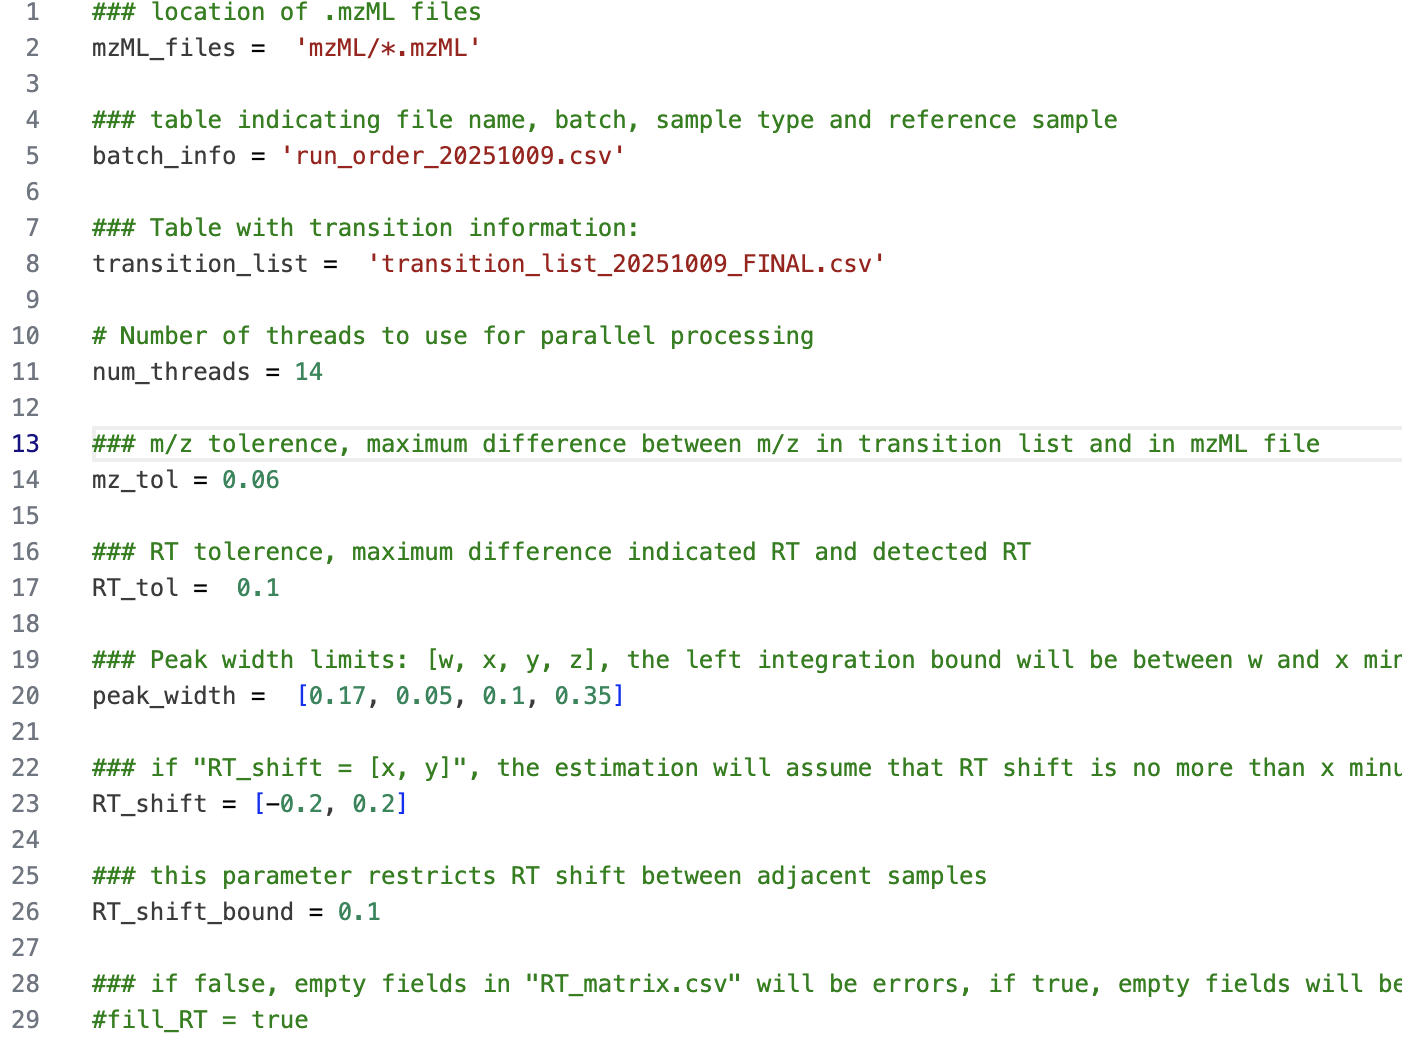
\includegraphics[width=1\linewidth,height=\textheight,keepaspectratio]{images/paste-5.png}

}

\caption{\textbf{Global settings file (param.txt).} Screenshot of the
param.txt file used for this dataset, showing all configured parameters
and their values.}

\end{figure}%

\subsubsection{Sample Table}\label{sample-table}

The sample table, provided as a CSV file, defines which samples are
processed and specifies sample-specific definitions and settings. Data
files to be processed must be listed by file name with the .mzML
extension in column A (file name). Samples designated as retention time
reference anchors are indicated with an x in column D (reference). The
sample type for each sample is defined in column C (sample\_type) using
the
\href{https://slinghub.github.io/MRMhub/articles/02_keydataids.html\#qc-types-sample-types}{MRMhub
QC type} nomenclature. Defining sample types is optional, INTEGRATOR
distinguishes only between blanks (identified by the presence of the
text \texttt{BLK}), and non-blanks. The sample type is, however,
included in the exported integration results. The batch identifier in
column B (batch) is not used by INTEGRATOR but is included in the
exported results.

\begin{figure}[H]

{\centering 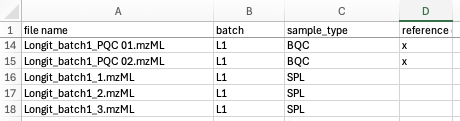
\includegraphics[width=1\linewidth,height=\textheight,keepaspectratio]{images/paste-1.png}

}

\caption{\textbf{Sample Table.} Screenshot of a portion of the CSV file
used for this dataset (run\_order\_20251009.csv). Two samples are
selected as RT reference samples.}

\end{figure}%

\subsubsection{Feature/Transition Table}\label{featuretransition-table}

The feature and transition table, provided as a CSV file, specifies the
transitions to be extracted from the mzML files and the features (peaks)
to be integrated from each transition (chromatogram).

Each transition is defined by the m/z values in the Precursor Ion and
Product Ion columns and must be assigned a name in the Transition Name
column. Ideally these m/z values exactly match those present in the mzML
files, however, transitions are identified based on the provided m/z
values and the tolerance specified by the mz\_tol parameter in param.txt
(default 0.06). Each feature must have a unique Compound Name and an
expected retention time (RT, in minutes). Multiple features may be
defined for the same transition, in which case the transition
information (m/z values and Transition Name) is repeated. The
corresponding internal standard feature for each feature (column ISTD)
is optional. The ISTD values are currently not used by the INTEGRATOR,
but are included in the exported integration results.

\begin{figure}[H]

{\centering 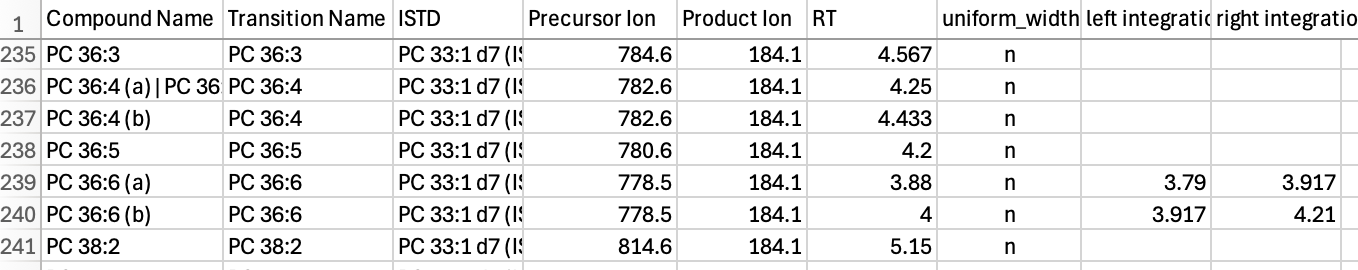
\includegraphics[width=1\linewidth,height=\textheight,keepaspectratio]{images/paste-6.png}

}

\caption{\textbf{Feature/Transition Table.} Screenshot of a portion of
the CSV file (transition\_list\_20251009\_Final.csv) used for this
dataset. Fixed integration borders were set for two adjacent features to
ensure correct integration.}

\end{figure}%

By default, peak integration is performed automatically on the basis of
the expected RT and the global peak\_width and RT\_tol settings. The
default automatic integration can be modified by feature-specific
settings. If uniform\_width is set to \textbf{\texttt{y}}, the median RT
for each left and right border is calculated from all non-Blank samples
and applied to all samples, including blanks. This option was not used
for the present dataset. Feature-specific peak width settings (column
`peak\_width') were not using for this example. Left integration bound
and right integration bound, if set, define fixed RTs for the left
and/or right peak borders. Fixed borders overwrite automatically derived
borders, including those determined when `uniform\_width' is set to
\textbf{\texttt{y}}, and they shift with the determined RT shifts. For
this dataset, fixed borders were applied for some features that were
poorly separated from adjacent peaks or that had noisy chromatograms to
ensure correct and consistent integration, for example PC 36:6. In some
other cases, isomers were intentionally co-integrated, such as the LPC
and LPE internal standards (see figure below).

The feature and transition table used in this workflow was optimized for
an earlier version of INTEGRATOR. Some feature-specific integration
settings included in that table may not be necessary with newer versions
of the software.

\begin{figure}[H]

{\centering \pandocbounded{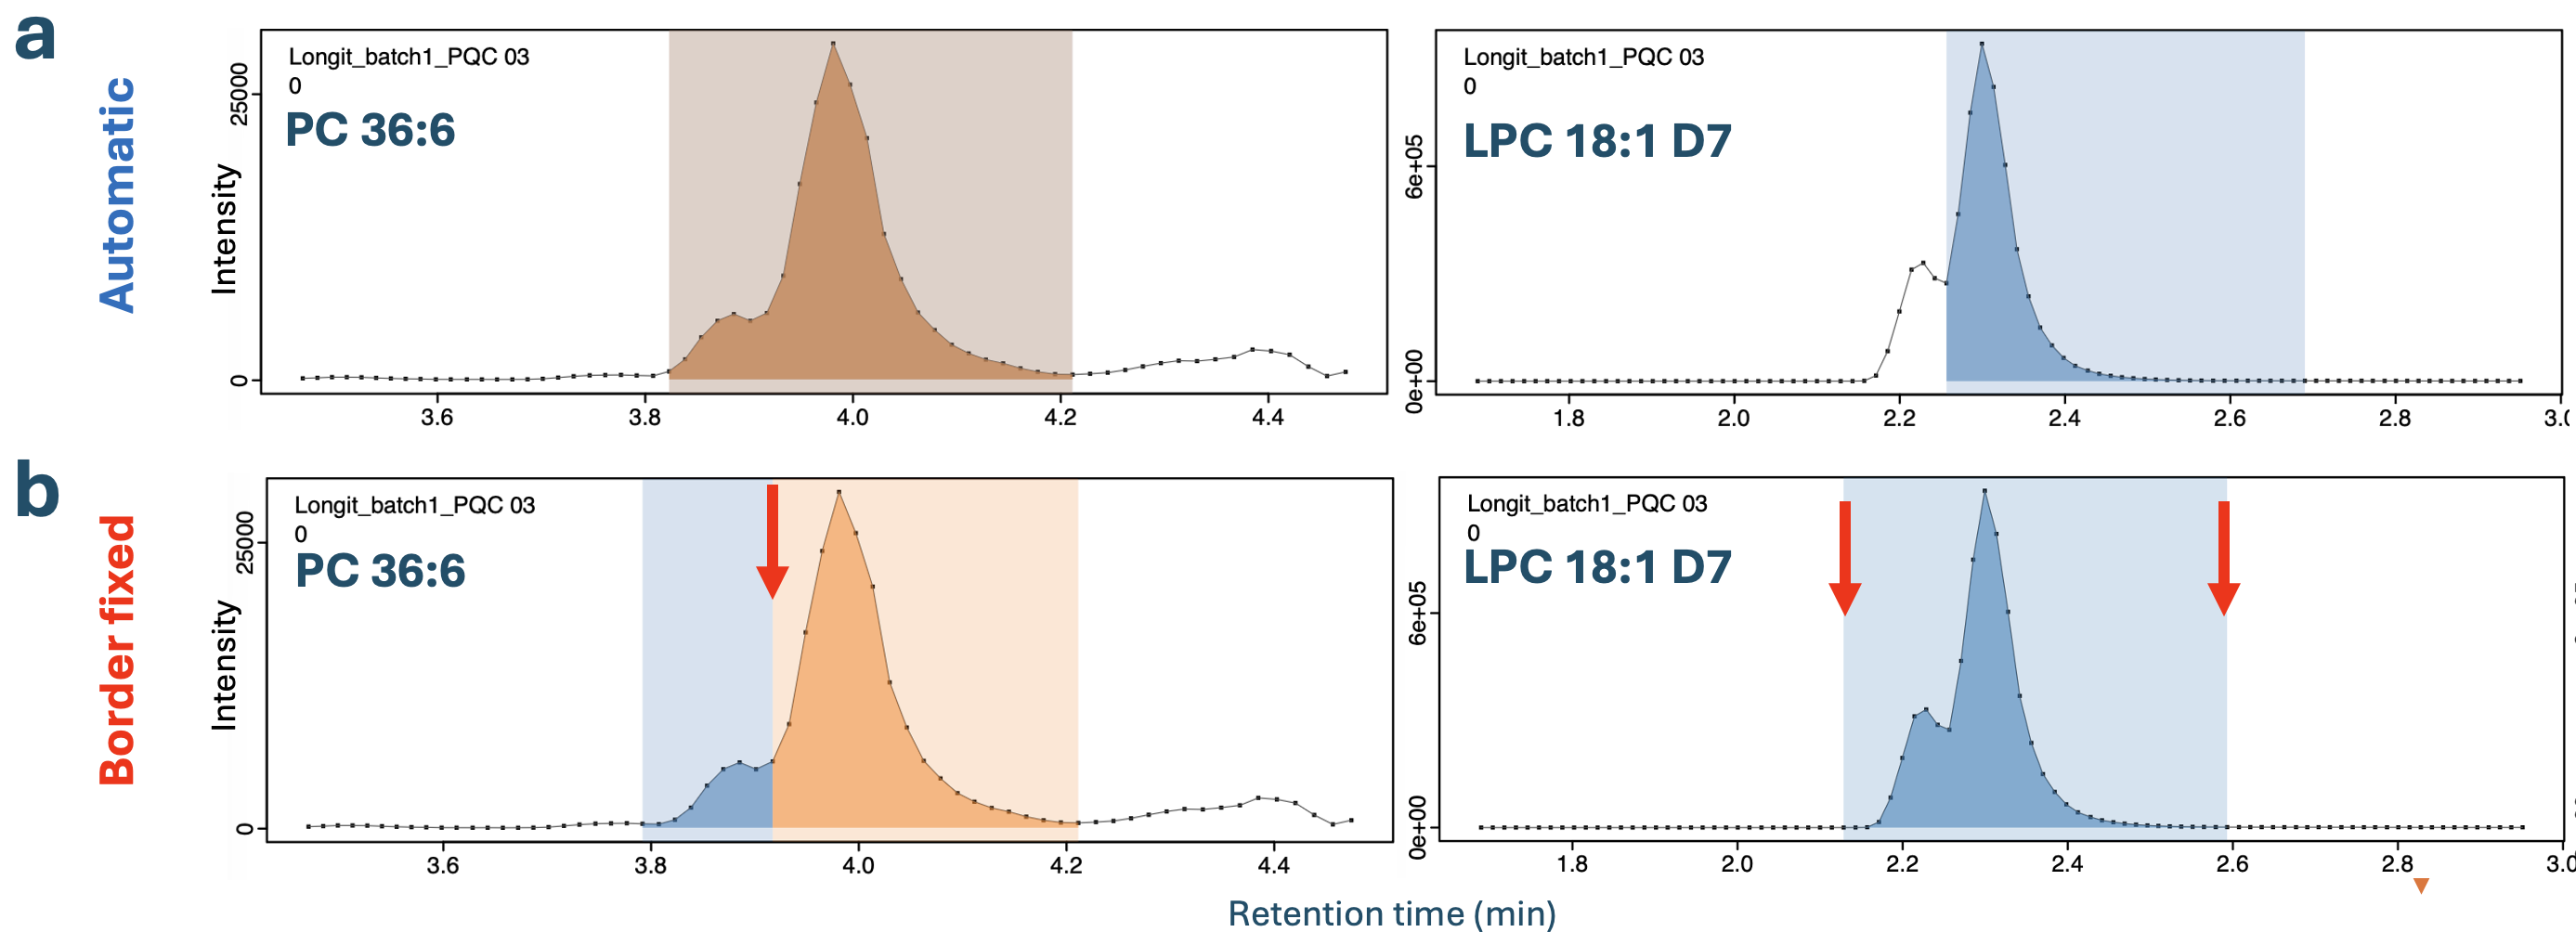
\includegraphics[keepaspectratio]{images/SupplCode1_Image1.png}}

}

\caption{\textbf{Examples of manually set peak boundaries for
MRMhub-INTEGRATOR}. (a) Automatic integration resulting in
co-integration of both overlapping peaks (PC 36:6) or integration of
only one peak (LPC 18:1 D7). (b) The same features integrated with fixed
boundaries for one and two peak boundaries, respectively. Red arrows
indicate feature-specific fixed integration border(s).}

\end{figure}%

\subsection{Running MRMhub-INTEGRATOR}\label{running-mrmhub-integrator}

After preparing all input files, the mrmhub application is started.
Steps 1 to 4 then run consecutively without further input to perform
peak detection, peak picking, integration, and export of data and PDF
results. The integration results are reported in the generated file
`long.csv', a long-format table that includes peak areas, actual
retention time, peak width, and other metadata. This data file will be
used for subsequent data postprocessing (see the following section). A
wide-format table with peak areas is available as `quant\_raw.csv'. PDFs
of the integrated transitions are available in the by\_* folders. See
the \hyperref[0]{INTEGRATOR Manual}for more details.

\begin{figure}[H]

{\centering 
\includegraphics[width=6.33333in,height=\textheight,keepaspectratio]{data/dataset-3/images/paste-3.png}

}

\caption{MRMhub-INTEGRATOR application.}

\end{figure}%

\subsection{Review of peak
integration}\label{review-of-peak-integration}

The peak integration results were inspected for all features across
samples using the generated PDFs (see above). For new methods or panels,
this review and the subsequent optimization of global and
feature-specific integration settings may require several iterations.
Once the parameters have been optimized, the global settings and the
feature table can typically be reused with only little tweaking,
provided the assay and instrument performance are reasonable consistent.

\section{Data Postprocessing: Quantification, Quality Control and
Reporting}\label{data-postprocessing-quantification-quality-control-and-reporting}

The postprocessing of the data obtained from the peak integration above
are conducted using MRMhun-QUANT, which is implemnted as the \{mrmhub\}
R package. A \href{https://quarto.org/}{Quarto} computational notebook
is used the run, document and report the data post processing.

\subsection{Setting up a Quarto Notebook and Installation of
\{mrmhub\}}\label{setting-up-a-quarto-notebook-and-installation-of-mrmhub}

A \href{https://quarto.org/}{Quarto} notebook can be created in tools
such as \href{https://posit.co/download/rstudio-desktop/}{RStudio},
\href{https://code.visualstudio.com}{VS Code}, or
\href{https://positron.posit.co}{Positon}. A
\href{https://cran.r-project.org}{installation of R}(Version
\textgreater= 4.2) needs to be present as well. Install or update the
\{mrmhub\} package by running following code in the R console, which
also installs two other R packages used in this workflow.

\begin{Shaded}
\begin{Highlighting}[]
\ControlFlowTok{if}\NormalTok{ (}\SpecialCharTok{!}\FunctionTok{require}\NormalTok{(}\StringTok{"remotes"}\NormalTok{)) }\FunctionTok{install.packages}\NormalTok{(}\StringTok{"remotes"}\NormalTok{)}
\NormalTok{remotes}\SpecialCharTok{::}\FunctionTok{install\_github}\NormalTok{(}\StringTok{"SLINGhub/MRMhub"}\NormalTok{, }\AttributeTok{subdir =} \StringTok{"quant"}\NormalTok{)}
\FunctionTok{install.packages}\NormalTok{(}\StringTok{"here"}\NormalTok{) }\CommentTok{\# Used for parallel processing}
\end{Highlighting}
\end{Shaded}

The Quarto notebook code generated in this example workflow is available
from \url{https://github.com/SLINGhub/MRMhub-workflows} (file
Dataset1.qmd). In the subsequent section, the data postprocessing is
encoded and documented step-by-step into the notebook as individual code
chunks using \{mrmhub\} functions. For many of the plots, the plots is
first assigned to a variable as the plots are also used to generate
figures for a manuscript (see code at the end of the notebook). In some
code cuncks addtional R code was used im order to show specific examples
rather then comprehnsive reports.

\subsection{Postprocessing workflow}\label{postprocessing-workflow}

\subsubsection{\texorpdfstring{Load \texttt{mrmhub} and other required
packages}{Load mrmhub and other required packages}}\label{load-mrmhub-and-other-required-packages}

\begin{Shaded}
\begin{Highlighting}[]
\FunctionTok{library}\NormalTok{(mrmhub)}
\FunctionTok{library}\NormalTok{(mirai)  }\CommentTok{\# Used for parallel processing}
\end{Highlighting}
\end{Shaded}

\subsubsection{Import the MRMhub-INTEGRATOR results (initial version of
the
dataset)}\label{import-the-mrmhub-integrator-results-initial-version-of-the-dataset}

We import the results of the initial peak integration iteration
obntained with the INTEGRATOR workflow, described in the previous
section. The corresponding original result file `long.csv' has been
renamed to `sPerfect\_LongCirc\_MRMkit\_Initial.csv'. The results
contain peak areas (\texttt{intensity}), retention time (\texttt{rt}),
and peak full width at half maximum (\texttt{fwhm}). Available metadata,
i.e., sample type, acquisition time stamp, precursor and product m/z
values are imported as well (\texttt{import\_metadata\ =\ TRUE}). The
data is stored in a \texttt{MRMhubExperiment} object, which will be used
in subsequent steps as data object (container).

\begin{Shaded}
\begin{Highlighting}[]
\NormalTok{data\_path }\OtherTok{\textless{}{-}} \StringTok{"./data/dataset{-}1/data/sPerfect\_LongCirc\_MRMkit\_Initial.csv"}
\NormalTok{mexp\_initial }\OtherTok{\textless{}{-}} \FunctionTok{MRMhubExperiment}\NormalTok{()}
\NormalTok{mexp\_initial }\OtherTok{\textless{}{-}} \FunctionTok{import\_data\_mrmhub}\NormalTok{(mexp\_initial, data\_path, }\AttributeTok{import\_metadata =} \ConstantTok{TRUE}\NormalTok{)                       }
\CommentTok{\#\textgreater{} v Imported 937 analyses with 503 features}
\CommentTok{\#\textgreater{} i \textasciigrave{}feature\_area\textasciigrave{} selected as default feature intensity. Modify with \textasciigrave{}set\_intensity\_var()\textasciigrave{}.}
\CommentTok{\#\textgreater{} v Analysis metadata associated with 937 analyses.}
\CommentTok{\#\textgreater{} v Feature metadata associated with 503 features.}
\end{Highlighting}
\end{Shaded}

\subsubsection{Analytical design and
timeline}\label{analytical-design-and-timeline}

The following plot provides an overview of the analysis structure,
detailing the types and sequence of QC samples analyzed. It also shows
information on the start and end dates, total duration, and median run
time for each sample. Setting \texttt{show\_timestamp\ =\ TRUE} in the
code below will plot the absolute dates as the x-axis, showing three
short interruptions, and the last 4 batches were measured approximately
one year later.

\begin{Shaded}
\begin{Highlighting}[]
\NormalTok{fig4a }\OtherTok{\textless{}{-}} \FunctionTok{plot\_runsequence}\NormalTok{(}
\NormalTok{  mexp\_initial, }
  \AttributeTok{show\_batches =} \ConstantTok{TRUE}\NormalTok{, }
  \AttributeTok{qc\_types =} \FunctionTok{c}\NormalTok{(}\StringTok{"SPL"}\NormalTok{, }\StringTok{"BQC"}\NormalTok{, }\StringTok{"TQC"}\NormalTok{, }\StringTok{"PBLK"}\NormalTok{, }\StringTok{"UBLK"}\NormalTok{, }\StringTok{"RQC"}\NormalTok{, }\StringTok{"SBLK"}\NormalTok{, }\StringTok{"LTR"}\NormalTok{),}
  \AttributeTok{batch\_zebra\_stripe =} \ConstantTok{TRUE}\NormalTok{, }
  \AttributeTok{base\_font\_size =} \DecValTok{6}\NormalTok{,}
  \AttributeTok{batch\_fill\_color =} \StringTok{"\#fffbdb"}\NormalTok{, }
  \AttributeTok{segment\_linewidth =} \FloatTok{0.5}\NormalTok{,}
  \AttributeTok{show\_timestamp =} \ConstantTok{FALSE}\NormalTok{) }\SpecialCharTok{+}
\FunctionTok{theme}\NormalTok{(}\AttributeTok{plot.title =} \FunctionTok{element\_text}\NormalTok{(}\AttributeTok{size =} \DecValTok{5}\NormalTok{))}
\NormalTok{fig4a}
\end{Highlighting}
\end{Shaded}

\includegraphics[width=1\linewidth,height=\textheight,keepaspectratio]{Dataset1_files/figure-pdf/chunk05-runsequence-plot-1.pdf}

\subsubsection{4. Overall trends and possible
outliers}\label{overall-trends-and-possible-outliers}

To examine overall technical trends and issues affecting most analytes
(features), the Relative Log Abundance (RLA) plot is useful (De Livera
et al., 2015 (Livera et al. 2015)). In an RLA plot, each feature is
normalised to the across-sample or within-batch median and the resulting
values are shown as boxplots for each sample. This visualization helps
identify technical problems such as pipetting errors, sample loss, or
changes in injection volume or instrument sensitivity. First, an
overview of all analyses (runs) is plotted.

\begin{Shaded}
\begin{Highlighting}[]
\FunctionTok{plot\_rla\_boxplot}\NormalTok{(}
  \AttributeTok{data =}\NormalTok{ mexp\_initial,}
  \AttributeTok{rla\_type\_batch =} \FunctionTok{c}\NormalTok{(}\StringTok{"within"}\NormalTok{),}
  \AttributeTok{variable =} \StringTok{"intensity"}\NormalTok{,}
  \AttributeTok{qc\_types =} \FunctionTok{c}\NormalTok{(}\StringTok{"BQC"}\NormalTok{, }\StringTok{"SPL"}\NormalTok{, }\StringTok{"LTR"}\NormalTok{, }\StringTok{"TQC"}\NormalTok{, }\StringTok{"RQC"}\NormalTok{, }\StringTok{"PBLK"}\NormalTok{),  }
  \AttributeTok{filter\_data =} \ConstantTok{FALSE}\NormalTok{, }
  \CommentTok{\#analysis\_range = get\_batch\_boundaries(myexp, batch\_indices = c(5,6)), }
  \AttributeTok{y\_lim =} \FunctionTok{c}\NormalTok{(}\SpecialCharTok{{-}}\DecValTok{3}\NormalTok{,}\DecValTok{3}\NormalTok{),}
  \AttributeTok{show\_timestamp =} \ConstantTok{FALSE}\NormalTok{,}
  \AttributeTok{outlier\_method =} \StringTok{"iqr"}\NormalTok{,}
  \AttributeTok{outlier\_k =} \FloatTok{1.5}\NormalTok{,}
  \AttributeTok{base\_font\_size =} \DecValTok{6}\NormalTok{,}
  \AttributeTok{outlier\_exclude =} \ConstantTok{FALSE}\NormalTok{, }
  \AttributeTok{x\_gridlines =} \ConstantTok{FALSE}\NormalTok{,}
  \AttributeTok{batch\_zebra\_stripe =} \ConstantTok{FALSE}\NormalTok{,}
  \AttributeTok{linewidth =} \FloatTok{0.1}\NormalTok{, }\AttributeTok{show\_plot =} \ConstantTok{TRUE}\NormalTok{)}
\CommentTok{\#\textgreater{} i Found 26 outliers in the 919 shown analyses}
\end{Highlighting}
\end{Shaded}

\includegraphics[width=1\linewidth,height=\textheight,keepaspectratio]{Dataset1_files/figure-pdf/chunk06-rla-plot-overview-1.png}

A zoom-in reveals that the engogenous (non-ISTD) feratures of one QC
sample type, the LTRs (long-term reference) have in average an
approximately 1/2 lower intensity compared to other samples.

\begin{Shaded}
\begin{Highlighting}[]
\CommentTok{\# An outlier sample, discussed later, will be excluded here}
\CommentTok{\# for demontration purposes.}

\NormalTok{mexp\_initial\_temp }\OtherTok{\textless{}{-}}\NormalTok{ mexp\_initial}
\NormalTok{mexp\_initial\_temp  }\OtherTok{\textless{}{-}} \FunctionTok{exclude\_analyses}\NormalTok{(}
\NormalTok{  mexp\_initial\_temp, }
  \AttributeTok{analyses =} \StringTok{"Longit\_batch6\_51"}\NormalTok{, }
  \AttributeTok{clear\_existing =} \ConstantTok{TRUE}\NormalTok{)}
\CommentTok{\#\textgreater{} i 1 analyses were excluded for downstream processing. Please reprocess data.}
\NormalTok{res }\OtherTok{\textless{}{-}} \FunctionTok{plot\_rla\_boxplot}\NormalTok{(}
  \AttributeTok{data =}\NormalTok{ mexp\_initial\_temp,}
  \AttributeTok{rla\_type\_batch =} \FunctionTok{c}\NormalTok{(}\StringTok{"across"}\NormalTok{),}
  \AttributeTok{variable =} \StringTok{"intensity"}\NormalTok{,}
  \AttributeTok{qc\_types =} \FunctionTok{c}\NormalTok{(}\StringTok{"BQC"}\NormalTok{, }\StringTok{"SPL"}\NormalTok{, }\StringTok{"LTR"}\NormalTok{, }\StringTok{"TQC"}\NormalTok{, }\StringTok{"RQC"}\NormalTok{), }
  \AttributeTok{filter\_data =} \ConstantTok{FALSE}\NormalTok{, }
  \AttributeTok{exclude\_feature\_filter =} \StringTok{"ISTD"}\NormalTok{,}
  \AttributeTok{plot\_range =}\FunctionTok{c}\NormalTok{(}\DecValTok{595}\NormalTok{,}\DecValTok{696}\NormalTok{),}
  \AttributeTok{y\_lim =} \FunctionTok{c}\NormalTok{(}\SpecialCharTok{{-}}\DecValTok{2}\NormalTok{,}\FloatTok{1.5}\NormalTok{),}
  \AttributeTok{include\_istd =} \ConstantTok{FALSE}\NormalTok{, }
  \AttributeTok{include\_qualifier =} \ConstantTok{FALSE}\NormalTok{,}
  \AttributeTok{min\_feature\_intensity =} \DecValTok{500}\NormalTok{,}
  \AttributeTok{show\_timestamp =} \ConstantTok{FALSE}\NormalTok{,}
  \AttributeTok{outlier\_method =} \StringTok{"iqr"}\NormalTok{,}
  \AttributeTok{outlier\_k =} \FloatTok{1.5}\NormalTok{,}
  \CommentTok{\#outlier\_k = c({-}1, 1),}
  \AttributeTok{outlier\_exclude =} \ConstantTok{FALSE}\NormalTok{, }
  \AttributeTok{x\_gridlines =} \ConstantTok{FALSE}\NormalTok{,}
  \AttributeTok{batch\_zebra\_stripe =} \ConstantTok{FALSE}\NormalTok{,}
  \AttributeTok{base\_font\_size =} \DecValTok{6}\NormalTok{,}
  \AttributeTok{show\_plot =} \ConstantTok{FALSE}\NormalTok{, }
  \AttributeTok{linewidth =} \FloatTok{0.1}
\NormalTok{)}
\CommentTok{\#\textgreater{} i Found 19 outliers in the 914 shown analyses}
\NormalTok{fig4b }\OtherTok{\textless{}{-}}\NormalTok{ res}\SpecialCharTok{$}\NormalTok{plot}
\NormalTok{fig4b}
\end{Highlighting}
\end{Shaded}

\includegraphics[width=1\linewidth,height=\textheight,keepaspectratio]{Dataset1_files/figure-pdf/chunk07-rla-plot-zoomin-analyte-only-1.png}

Now we plot the distributions of the ISTDs only. We see that also they
also have an approximately 1/2 lower intensity in the LTR samples
compared to the other samples. This may suggest that the measured sample
amount was lower for the LTR samples, or that twice the amount of
extraction solvent was added, both of which will lead to reduction of
all features, including ISTDs.

\begin{Shaded}
\begin{Highlighting}[]
\NormalTok{extfig2b }\OtherTok{\textless{}{-}} \FunctionTok{plot\_rla\_boxplot}\NormalTok{(}
  \AttributeTok{data =}\NormalTok{ mexp\_initial,}
  \AttributeTok{rla\_type\_batch =} \FunctionTok{c}\NormalTok{(}\StringTok{"across"}\NormalTok{),}
  \AttributeTok{variable =} \StringTok{"intensity"}\NormalTok{,}
  \AttributeTok{qc\_types =} \FunctionTok{c}\NormalTok{(}\StringTok{"BQC"}\NormalTok{, }\StringTok{"SPL"}\NormalTok{, }\StringTok{"LTR"}\NormalTok{, }\StringTok{"TQC"}\NormalTok{, }\StringTok{"RQC"}\NormalTok{, }\StringTok{"PBLK"}\NormalTok{), }
  \AttributeTok{filter\_data =} \ConstantTok{FALSE}\NormalTok{, }
  \AttributeTok{include\_feature\_filter =} \StringTok{"ISTD"}\NormalTok{,}
  \AttributeTok{plot\_range =}\FunctionTok{c}\NormalTok{(}\DecValTok{595}\NormalTok{,}\DecValTok{696}\NormalTok{),}
  \AttributeTok{y\_lim =} \FunctionTok{c}\NormalTok{(}\SpecialCharTok{{-}}\DecValTok{2}\NormalTok{,}\FloatTok{1.5}\NormalTok{),}
  \AttributeTok{include\_istd =} \ConstantTok{TRUE}\NormalTok{, }
  \AttributeTok{include\_qualifier =} \ConstantTok{FALSE}\NormalTok{,}
  \AttributeTok{min\_feature\_intensity =} \DecValTok{500}\NormalTok{,}
  \AttributeTok{show\_timestamp =} \ConstantTok{FALSE}\NormalTok{,}
  \AttributeTok{outlier\_method =} \StringTok{"iqr"}\NormalTok{,}
  \AttributeTok{outlier\_k =} \FloatTok{1.5}\NormalTok{,}
  \AttributeTok{outlier\_exclude =} \ConstantTok{FALSE}\NormalTok{, }
  \AttributeTok{x\_gridlines =} \ConstantTok{FALSE}\NormalTok{,}
  \AttributeTok{batch\_zebra\_stripe =} \ConstantTok{FALSE}\NormalTok{,}
  \AttributeTok{show\_plot =} \ConstantTok{FALSE}\NormalTok{,}
  \AttributeTok{base\_font\_size =} \DecValTok{8}\NormalTok{,}
  \AttributeTok{linewidth =} \FloatTok{0.2}
\NormalTok{)}\SpecialCharTok{$}\NormalTok{plot}
\CommentTok{\#\textgreater{} i Found 13 outliers in the 919 shown analyses}
\NormalTok{extfig2b}
\end{Highlighting}
\end{Shaded}

\includegraphics[width=1\linewidth,height=\textheight,keepaspectratio]{Dataset1_files/figure-pdf/chunk08b-rla-plot-zoomin-istd-only-1.png}

A further, detailed, batch-by-batch inspection, revealed that in batch
6, the sample ``Longit\_batch6\_51'' at position 464 had significantly
lower intensities of non-ISTD feature, with intensities comparable to
Blanks.

\begin{Shaded}
\begin{Highlighting}[]
\NormalTok{extfig2c }\OtherTok{\textless{}{-}} \FunctionTok{plot\_rla\_boxplot}\NormalTok{(}
  \AttributeTok{data =}\NormalTok{ mexp\_initial,}
  \AttributeTok{rla\_type\_batch =} \FunctionTok{c}\NormalTok{(}\StringTok{"across"}\NormalTok{),}
  \AttributeTok{variable =} \StringTok{"intensity"}\NormalTok{,}
  \AttributeTok{qc\_types =} \FunctionTok{c}\NormalTok{(}\StringTok{"BQC"}\NormalTok{, }\StringTok{"SPL"}\NormalTok{, }\StringTok{"LTR"}\NormalTok{, }\StringTok{"TQC"}\NormalTok{, }\StringTok{"RQC"}\NormalTok{, }\StringTok{"PBLK"}\NormalTok{), }
  \AttributeTok{filter\_data =} \ConstantTok{FALSE}\NormalTok{, }
  \AttributeTok{plot\_range =} \FunctionTok{c}\NormalTok{(}\DecValTok{430}\NormalTok{,}\DecValTok{522}\NormalTok{),}
  \AttributeTok{y\_lim =} \FunctionTok{c}\NormalTok{(}\SpecialCharTok{{-}}\DecValTok{10}\NormalTok{,}\FloatTok{1.5}\NormalTok{),}
  \AttributeTok{include\_istd =}  \ConstantTok{FALSE}\NormalTok{, }
  \AttributeTok{exclude\_feature\_filter =} \StringTok{"ISTD"}\NormalTok{,}
  \AttributeTok{include\_qualifier =} \ConstantTok{FALSE}\NormalTok{,}
  \AttributeTok{min\_feature\_intensity =} \DecValTok{500}\NormalTok{,}
  \AttributeTok{show\_timestamp =} \ConstantTok{FALSE}\NormalTok{,}
  \AttributeTok{outlier\_method =} \StringTok{"iqr"}\NormalTok{,}
  \AttributeTok{outlier\_k =} \FloatTok{1.5}\NormalTok{,}
  \AttributeTok{outlier\_exclude =} \ConstantTok{FALSE}\NormalTok{, }
  \AttributeTok{x\_gridlines =} \ConstantTok{FALSE}\NormalTok{,}
  \AttributeTok{batch\_zebra\_stripe =} \ConstantTok{FALSE}\NormalTok{,}
  \AttributeTok{base\_font\_size =} \DecValTok{6}\NormalTok{,}
  \AttributeTok{show\_plot =} \ConstantTok{FALSE}\NormalTok{,}
  \AttributeTok{linewidth =} \FloatTok{0.2}\NormalTok{)}\SpecialCharTok{$}\NormalTok{plot }\SpecialCharTok{+}
    \FunctionTok{theme}\NormalTok{(}
      \AttributeTok{strip.text =}\NormalTok{ ggplot2}\SpecialCharTok{::}\FunctionTok{element\_text}\NormalTok{(}\AttributeTok{size =} \DecValTok{8}\NormalTok{),}
      \CommentTok{\#aspect.ratio = 0.9,}
      \AttributeTok{legend.position =} \StringTok{"inside"}\NormalTok{,}
      \AttributeTok{axis.text =} \FunctionTok{element\_text}\NormalTok{(}\AttributeTok{size =} \DecValTok{8}\NormalTok{),}
      \CommentTok{\#legend.direction = "vertical", }
      \AttributeTok{legend.text =} \FunctionTok{element\_text}\NormalTok{(}\AttributeTok{size =} \DecValTok{8}\NormalTok{), }
      \AttributeTok{legend.title =} \FunctionTok{element\_text}\NormalTok{(}\AttributeTok{size =} \DecValTok{8}\NormalTok{),}
      \AttributeTok{legend.key.size =} \FunctionTok{unit}\NormalTok{(}\DecValTok{8}\NormalTok{, }\StringTok{"pt"}\NormalTok{), }
      \AttributeTok{legend.position.inside =} \FunctionTok{c}\NormalTok{(}\FloatTok{0.3}\NormalTok{, }\FloatTok{0.32}\NormalTok{))}
\CommentTok{\#\textgreater{} i Found 20 outliers in the 919 shown analyses}
\NormalTok{extfig2c}
\end{Highlighting}
\end{Shaded}

\includegraphics[width=1\linewidth,height=\textheight,keepaspectratio]{Dataset1_files/figure-pdf/chunk09-rla-plot-zoomin-batch6-1.png}

However, the ISTDs signals were comparable with other samples. This
likely suggests that this study sample was not added to the extraction
vial before extraction. The sample will be excluded from further
analysis.

\begin{Shaded}
\begin{Highlighting}[]
\NormalTok{mexp\_initial\_temp2 }\OtherTok{\textless{}{-}}\NormalTok{ mexp\_initial}
\NormalTok{mexp\_initial\_temp2}\SpecialCharTok{@}\NormalTok{dataset }\OtherTok{\textless{}{-}}\NormalTok{ mexp\_initial\_temp2}\SpecialCharTok{@}\NormalTok{dataset }\SpecialCharTok{|\textgreater{}} \FunctionTok{filter}\NormalTok{(is\_istd)}

\NormalTok{extfig2d }\OtherTok{\textless{}{-}} \FunctionTok{plot\_rla\_boxplot}\NormalTok{(}
  \AttributeTok{data =}\NormalTok{ mexp\_initial\_temp2,}
  \AttributeTok{rla\_type\_batch =} \FunctionTok{c}\NormalTok{(}\StringTok{"across"}\NormalTok{),}
  \AttributeTok{variable =} \StringTok{"intensity"}\NormalTok{,}
  \AttributeTok{qc\_types =} \FunctionTok{c}\NormalTok{(}\StringTok{"BQC"}\NormalTok{, }\StringTok{"SPL"}\NormalTok{, }\StringTok{"LTR"}\NormalTok{, }\StringTok{"TQC"}\NormalTok{, }\StringTok{"RQC"}\NormalTok{, }\StringTok{"PBLK"}\NormalTok{), }
  \AttributeTok{filter\_data =} \ConstantTok{FALSE}\NormalTok{, }
  \AttributeTok{plot\_range =} \FunctionTok{c}\NormalTok{(}\DecValTok{430}\NormalTok{,}\DecValTok{522}\NormalTok{),}
  \AttributeTok{y\_lim =} \FunctionTok{c}\NormalTok{(}\SpecialCharTok{{-}}\DecValTok{10}\NormalTok{, }\FloatTok{1.5}\NormalTok{),}
  \AttributeTok{include\_istd =} \ConstantTok{TRUE}\NormalTok{, }
  \AttributeTok{include\_feature\_filter =} \StringTok{"ISTD"}\NormalTok{,}
  \AttributeTok{include\_qualifier =} \ConstantTok{FALSE}\NormalTok{,}
  \AttributeTok{min\_feature\_intensity =} \DecValTok{500}\NormalTok{,}
  \AttributeTok{show\_timestamp =} \ConstantTok{FALSE}\NormalTok{,}
  \AttributeTok{outlier\_method =} \StringTok{"iqr"}\NormalTok{,}
  \AttributeTok{outlier\_k =} \FloatTok{1.5}\NormalTok{,}
  \AttributeTok{outlier\_exclude =} \ConstantTok{FALSE}\NormalTok{, }
  \AttributeTok{x\_gridlines =} \ConstantTok{FALSE}\NormalTok{,}
  \AttributeTok{batch\_zebra\_stripe =} \ConstantTok{FALSE}\NormalTok{,}
  \AttributeTok{base\_font\_size =} \DecValTok{8}\NormalTok{,}
  \AttributeTok{show\_plot =} \ConstantTok{FALSE}\NormalTok{,}
  \AttributeTok{linewidth =} \FloatTok{0.2}\NormalTok{)}\SpecialCharTok{$}\NormalTok{plot }\SpecialCharTok{+}
    \FunctionTok{theme}\NormalTok{(}
    \AttributeTok{strip.text =}\NormalTok{ ggplot2}\SpecialCharTok{::}\FunctionTok{element\_text}\NormalTok{(}\AttributeTok{size =} \DecValTok{8}\NormalTok{),}
    \CommentTok{\#aspect.ratio = 0.9,}
    \AttributeTok{legend.position =} \StringTok{"inside"}\NormalTok{,}
    \AttributeTok{axis.text =} \FunctionTok{element\_text}\NormalTok{(}\AttributeTok{size =} \DecValTok{8}\NormalTok{),}
    \CommentTok{\#legend.direction = "vertical", }
    \AttributeTok{legend.text =} \FunctionTok{element\_text}\NormalTok{(}\AttributeTok{size =} \DecValTok{8}\NormalTok{), }
    \AttributeTok{legend.title =} \FunctionTok{element\_text}\NormalTok{(}\AttributeTok{size =} \DecValTok{8}\NormalTok{),}
    \AttributeTok{legend.key.size =} \FunctionTok{unit}\NormalTok{(}\DecValTok{8}\NormalTok{, }\StringTok{"pt"}\NormalTok{), }
    \AttributeTok{legend.position.inside =} \FunctionTok{c}\NormalTok{(}\FloatTok{0.3}\NormalTok{, }\FloatTok{0.32}\NormalTok{))}
\CommentTok{\#\textgreater{} i Found 20 outliers in the 919 shown analyses}
\NormalTok{extfig2d}
\end{Highlighting}
\end{Shaded}

\includegraphics[width=1\linewidth,height=\textheight,keepaspectratio]{Dataset1_files/figure-pdf/chunk09b-rla-plot-zoomin-batch6-1.png}

\subsection{Peak annotation QC}\label{peak-annotation-qc}

To check for potential peak picking errors during the peak integration
step (see section above), the retention time (RT) of lipid features is
plotted against the total carbon number and double bond number. This QC
plot reveals several potential peak picking errors, especially among the
SM, which are likely caused by erroneous picking of the isobaric
isotopologue peak of PCs.

To check for potential peak picking errors during the peak integration
step (see section above), the retention time (RT) of lipid features are
plotted against the total carbon count and double bond number. The
currently imported datas was the result of an interative process of data
review using the QC plot and curation, this actual dataset corresponds
to final dataset after curation.

Lipid species flagged as potential misannotations were manually
inspected in the chromatograms and compared with an online resource for
lipid RTs measured using the same LC-MS method
(https://metabolomics.baker.edu.au/method/lipids). These features were
deemed likely correct.

\begin{Shaded}
\begin{Highlighting}[]
\NormalTok{mexp\_initial }\OtherTok{\textless{}{-}} \FunctionTok{exclude\_analyses}\NormalTok{(mexp\_initial, }
                                  \AttributeTok{analyses =} \StringTok{"Longit\_batch6\_51"}\NormalTok{, }
                                  \AttributeTok{clear\_existing =} \ConstantTok{TRUE}\NormalTok{)}
\CommentTok{\#\textgreater{} i 1 analyses were excluded for downstream processing. Please reprocess data.}
\NormalTok{mexp\_temp }\OtherTok{\textless{}{-}}\NormalTok{ mexp\_initial}
\NormalTok{mexp\_temp}\SpecialCharTok{@}\NormalTok{dataset }\OtherTok{\textless{}{-}}\NormalTok{ mexp\_temp}\SpecialCharTok{@}\NormalTok{dataset }\SpecialCharTok{|\textgreater{}} \FunctionTok{filter}\NormalTok{(}\FunctionTok{str\_detect}\NormalTok{(feature\_id, }\StringTok{"\^{}PC }\SpecialCharTok{\textbackslash{}\textbackslash{}}\StringTok{d"}\NormalTok{))}

\NormalTok{fig4c }\OtherTok{\textless{}{-}} \FunctionTok{plot\_rt\_vs\_chain}\NormalTok{(}
\NormalTok{  mexp\_temp, }
  \AttributeTok{qc\_types =} \StringTok{"SPL"}\NormalTok{, }
  \AttributeTok{x\_var =} \StringTok{"total\_c"}\NormalTok{, }
  \AttributeTok{base\_font\_size =} \DecValTok{6}\NormalTok{) }\SpecialCharTok{+}
  \FunctionTok{theme}\NormalTok{( }
      \AttributeTok{legend.position =} \StringTok{"right"}\NormalTok{,}
      \AttributeTok{legend.direction =} \StringTok{"vertical"}\NormalTok{, }
      \AttributeTok{legend.text =} \FunctionTok{element\_text}\NormalTok{(}\AttributeTok{size =}\NormalTok{ base\_font\_size}\SpecialCharTok{*}\FloatTok{0.8}\NormalTok{), }
      \AttributeTok{legend.title =} \FunctionTok{element\_text}\NormalTok{(}\AttributeTok{size =}\NormalTok{ base\_font\_size}\SpecialCharTok{*}\FloatTok{0.8}\NormalTok{),}
      \AttributeTok{legend.key.size =} \FunctionTok{unit}\NormalTok{(base\_font\_size }\SpecialCharTok{*}\FloatTok{0.8}\NormalTok{, }\StringTok{"pt"}\NormalTok{), }
      \AttributeTok{legend.position.inside =} \FunctionTok{c}\NormalTok{(}\FloatTok{0.1}\NormalTok{, }\FloatTok{0.7}\NormalTok{)}
\NormalTok{      )  }
\CommentTok{\#\textgreater{} i The following features were flagged as potential annotation outliers: PC 30:0 (b), PC 32:1, PC 32:2, PC 38:3 (a)}
\NormalTok{fig4c}
\end{Highlighting}
\end{Shaded}

\includegraphics[width=1\linewidth,height=\textheight,keepaspectratio]{Dataset1_files/figure-pdf/chunk10-rt-vs-chain-1.pdf}

\subsection{7. Feature correlation
analysis}\label{feature-correlation-analysis}

As another check for potential peak picking errors, highly correlating
features are plotted.

\begin{Shaded}
\begin{Highlighting}[]
\CommentTok{\# this below is to exclude a sample that has a very low intensity for all features, see next steps for }
\CommentTok{\# details}
\CommentTok{\#| fig{-}format: png}
\CommentTok{\#| dpi: 600}
\NormalTok{mexp\_initial }\OtherTok{\textless{}{-}} \FunctionTok{exclude\_analyses}\NormalTok{(}
\NormalTok{  mexp\_initial, }
  \AttributeTok{analyses =} \StringTok{"Longit\_batch6\_51"}\NormalTok{, }
  \AttributeTok{clear\_existing =} \ConstantTok{TRUE}\NormalTok{)}
\CommentTok{\#\textgreater{} i 1 analyses were excluded for downstream processing. Please reprocess data.}
\NormalTok{fig4d }\OtherTok{\textless{}{-}} \FunctionTok{plot\_feature\_correlations}\NormalTok{(}
\NormalTok{  mexp\_initial, }
  \AttributeTok{variable =} \StringTok{"intensity"}\NormalTok{, }
  \AttributeTok{include\_feature\_filter =} \FunctionTok{c}\NormalTok{(}
    \StringTok{"Cer d18:1/24:0"}\NormalTok{, }\StringTok{"Cer d18:0/24:1"}\NormalTok{),}
  \AttributeTok{qc\_types =} \FunctionTok{c}\NormalTok{(}\StringTok{"SPL"}\NormalTok{, }\StringTok{"BQC"}\NormalTok{, }\StringTok{"TQC"}\NormalTok{), }
  \AttributeTok{cor\_min =} \FloatTok{0.1}\NormalTok{,}\AttributeTok{sort\_by\_corr =} \ConstantTok{TRUE}\NormalTok{, }\AttributeTok{return\_plot =} \ConstantTok{TRUE}\NormalTok{,}\AttributeTok{show\_progress =}\NormalTok{ F,}
  \AttributeTok{log\_scale =} \ConstantTok{FALSE}\NormalTok{, }\AttributeTok{cols\_page =} \DecValTok{1}\NormalTok{, }\AttributeTok{rows\_page =} \DecValTok{1}\NormalTok{, }
  \AttributeTok{font\_base\_size =} \DecValTok{6}\NormalTok{)[[}\DecValTok{1}\NormalTok{]] }\SpecialCharTok{+} 
  \FunctionTok{theme}\NormalTok{(}
    \AttributeTok{strip.text =}\NormalTok{ ggplot2}\SpecialCharTok{::}\FunctionTok{element\_text}\NormalTok{(}\AttributeTok{size =} \DecValTok{6}\NormalTok{),}
    \CommentTok{\#aspect.ratio = 0.9,}
    \AttributeTok{legend.position =} \StringTok{"inside"}\NormalTok{,}
    \AttributeTok{axis.text =} \FunctionTok{element\_text}\NormalTok{(}\AttributeTok{size =} \DecValTok{5}\NormalTok{),}
    \AttributeTok{legend.direction =} \StringTok{"vertical"}\NormalTok{, }
    \AttributeTok{legend.text =} \FunctionTok{element\_text}\NormalTok{(}\AttributeTok{size =} \DecValTok{6}\SpecialCharTok{*}\FloatTok{0.7}\NormalTok{), }
    \AttributeTok{legend.title =} \FunctionTok{element\_text}\NormalTok{(}\AttributeTok{size =} \DecValTok{6}\SpecialCharTok{*}\FloatTok{0.7}\NormalTok{),}
    \AttributeTok{legend.key.size =} \FunctionTok{unit}\NormalTok{(}\DecValTok{6} \SpecialCharTok{*}\FloatTok{0.7}\NormalTok{, }\StringTok{"pt"}\NormalTok{), }
    \AttributeTok{legend.position.inside =} \FunctionTok{c}\NormalTok{(}\FloatTok{0.9}\NormalTok{, }\FloatTok{0.12}\NormalTok{)}
\NormalTok{)  }
\CommentTok{\#\textgreater{} Generating plots (1 page)}
\NormalTok{fig4d}
\end{Highlighting}
\end{Shaded}

\includegraphics[width=1\linewidth,height=\textheight,keepaspectratio]{Dataset1_files/figure-pdf/chunk11-feature-correlation-1.pdf}

\subsection{8. Fix peak integration and re-import data
(V2)}\label{fix-peak-integration-and-re-import-data-v2}

We now went back to the MRMkit workflow and corrected the peak
integration errors The corrected data is available in the file
\texttt{sPerfect\_LongCirc\_MRMkit.csv}. We import the corrected data,
which we will use from now.

\begin{Shaded}
\begin{Highlighting}[]
\NormalTok{mexp }\OtherTok{\textless{}{-}} \FunctionTok{MRMhubExperiment}\NormalTok{()}
\NormalTok{mexp }\OtherTok{\textless{}{-}} \FunctionTok{import\_data\_mrmhub}\NormalTok{(}
\NormalTok{  mexp, }
  \StringTok{"./data/dataset{-}1/data/sPerfect\_LongCirc\_MRMkit\_Final.csv"}
\NormalTok{)}
\CommentTok{\#\textgreater{} v Imported 937 analyses with 482 features}
\CommentTok{\#\textgreater{} i \textasciigrave{}feature\_area\textasciigrave{} selected as default feature intensity. Modify with \textasciigrave{}set\_intensity\_var()\textasciigrave{}.}
\CommentTok{\#\textgreater{} v Analysis metadata associated with 937 analyses.}
\CommentTok{\#\textgreater{} v Feature metadata associated with 482 features.}
\end{Highlighting}
\end{Shaded}

We also directly plot the RT against chain lengths again, which confirms
that the peak picking errors seems to have been corrected.

\begin{Shaded}
\begin{Highlighting}[]
\NormalTok{extfig3a }\OtherTok{\textless{}{-}} \FunctionTok{plot\_rt\_vs\_chain}\NormalTok{(mexp\_initial, }\AttributeTok{qc\_types =} \StringTok{"SPL"}\NormalTok{, }\AttributeTok{x\_var =} \StringTok{"total\_c"}\NormalTok{, }\AttributeTok{base\_font\_size =} \DecValTok{6}\NormalTok{)}\SpecialCharTok{+}
  \FunctionTok{theme}\NormalTok{( }
      \AttributeTok{legend.position =} \StringTok{"right"}\NormalTok{,}
      \AttributeTok{legend.direction =} \StringTok{"vertical"}\NormalTok{, }
      \AttributeTok{legend.text =} \FunctionTok{element\_text}\NormalTok{(}\AttributeTok{size =}\NormalTok{ base\_font\_size}\SpecialCharTok{*}\FloatTok{0.8}\NormalTok{), }
      \AttributeTok{legend.title =} \FunctionTok{element\_text}\NormalTok{(}\AttributeTok{size =}\NormalTok{ base\_font\_size}\SpecialCharTok{*}\FloatTok{0.8}\NormalTok{),}
      \AttributeTok{legend.key.size =} \FunctionTok{unit}\NormalTok{(base\_font\_size }\SpecialCharTok{*}\FloatTok{0.8}\NormalTok{, }\StringTok{"pt"}\NormalTok{), }
      \AttributeTok{legend.position.inside =} \FunctionTok{c}\NormalTok{(}\FloatTok{0.1}\NormalTok{, }\FloatTok{0.7}\NormalTok{))}
\CommentTok{\#\textgreater{} i The following features were flagged as potential annotation outliers: DG 18:1\_20:0 [{-}18:1], DG 14:1\_20:0 [{-}20:0], LPC 17:1 (c), PC 30:0 (b), PC 32:1, PC 32:2, PC 38:3 (a), SM 41:1 (a), SM 40:1, SM 39:1, SM 44:2 M+2, SM 42:2, SM 36:2, SM 36:2 d9 (ISTD), SM 35:2, SM 32:2, SM 38:3|PC 33:1 d7 M+2, SM 34:3, TG 48:0 d5 (ISTD) [{-}16:0], TG O{-}51:2 [{-}18:1]}
\NormalTok{extfig3a  }
\end{Highlighting}
\end{Shaded}

\includegraphics[width=1\linewidth,height=\textheight,keepaspectratio]{Dataset1_files/figure-pdf/chunk13-rt-vs-chain-v2-1.pdf}

\begin{Shaded}
\begin{Highlighting}[]
\NormalTok{extfig3b }\OtherTok{\textless{}{-}} \FunctionTok{plot\_rt\_vs\_chain}\NormalTok{(mexp, }\AttributeTok{qc\_types =} \StringTok{"SPL"}\NormalTok{, }\AttributeTok{x\_var =} \StringTok{"total\_c"}\NormalTok{, }\AttributeTok{base\_font\_size =} \DecValTok{6}\NormalTok{)}\SpecialCharTok{+}
  \FunctionTok{theme}\NormalTok{( }
      \AttributeTok{legend.position =} \StringTok{"right"}\NormalTok{,}
      \AttributeTok{legend.direction =} \StringTok{"vertical"}\NormalTok{, }
      \AttributeTok{legend.text =} \FunctionTok{element\_text}\NormalTok{(}\AttributeTok{size =}\NormalTok{ base\_font\_size}\SpecialCharTok{*}\FloatTok{0.8}\NormalTok{), }
      \AttributeTok{legend.title =} \FunctionTok{element\_text}\NormalTok{(}\AttributeTok{size =}\NormalTok{ base\_font\_size}\SpecialCharTok{*}\FloatTok{0.8}\NormalTok{),}
      \AttributeTok{legend.key.size =} \FunctionTok{unit}\NormalTok{(base\_font\_size }\SpecialCharTok{*}\FloatTok{0.8}\NormalTok{, }\StringTok{"pt"}\NormalTok{), }
      \AttributeTok{legend.position.inside =} \FunctionTok{c}\NormalTok{(}\FloatTok{0.1}\NormalTok{, }\FloatTok{0.7}\NormalTok{))}
\CommentTok{\#\textgreater{} i The following features were flagged as potential annotation outliers: LPC 17:1 (c), SM 41:1 (a)}
\NormalTok{extfig3b}
\end{Highlighting}
\end{Shaded}

\includegraphics[width=1\linewidth,height=\textheight,keepaspectratio]{Dataset1_files/figure-pdf/chunk13-rt-vs-chain-v2-2.pdf}

\subsection{PCA to check for potential technical
outliers}\label{pca-to-check-for-potential-technical-outliers}

\begin{Shaded}
\begin{Highlighting}[]
\NormalTok{extfig4a }\OtherTok{\textless{}{-}} \FunctionTok{plot\_pca}\NormalTok{(}
  \AttributeTok{data =}\NormalTok{ mexp,}
  \AttributeTok{variable =} \StringTok{"intensity"}\NormalTok{,}
  \AttributeTok{filter\_data =} \ConstantTok{FALSE}\NormalTok{,}
  \AttributeTok{pca\_dims =} \FunctionTok{c}\NormalTok{(}\DecValTok{1}\NormalTok{,}\DecValTok{2}\NormalTok{),}
  \AttributeTok{labels\_threshold\_mad =} \DecValTok{4}\NormalTok{,}
  \AttributeTok{qc\_types =} \FunctionTok{c}\NormalTok{(}\StringTok{"SPL"}\NormalTok{, }\StringTok{"BQC"}\NormalTok{, }\StringTok{"TQC"}\NormalTok{, }\StringTok{"LTR"}\NormalTok{),}
  \AttributeTok{ellipse\_variable =} \StringTok{"qc\_type"}\NormalTok{,}
  \AttributeTok{log\_transform =} \ConstantTok{TRUE}\NormalTok{,}
  \AttributeTok{point\_size =} \DecValTok{1}\NormalTok{, }\AttributeTok{point\_alpha =} \FloatTok{0.7}\NormalTok{, }\AttributeTok{font\_base\_size =} \DecValTok{8}\NormalTok{, }\AttributeTok{ellipse\_alpha =} \FloatTok{0.3}\NormalTok{,}
  \AttributeTok{include\_istd =} \ConstantTok{FALSE}\NormalTok{,}\AttributeTok{show\_labels =} \ConstantTok{TRUE}\NormalTok{,}\AttributeTok{label\_font\_size =} \DecValTok{2}\NormalTok{,}
  \AttributeTok{shared\_labeltext\_hide =} \ConstantTok{NA}\NormalTok{)   }\SpecialCharTok{+} \FunctionTok{theme}\NormalTok{(}
    \AttributeTok{plot.title =} \FunctionTok{element\_blank}\NormalTok{(),}
    \AttributeTok{aspect.ratio =} \DecValTok{1}\NormalTok{,}
        \AttributeTok{legend.position =} \StringTok{"inside"}\NormalTok{,}
      \AttributeTok{legend.direction =} \StringTok{"vertical"}\NormalTok{, }
      \AttributeTok{legend.text =} \FunctionTok{element\_text}\NormalTok{(}\AttributeTok{size =} \DecValTok{9}\SpecialCharTok{*}\FloatTok{0.7}\NormalTok{), }
      \AttributeTok{legend.title =} \FunctionTok{element\_text}\NormalTok{(}\AttributeTok{size =} \DecValTok{9}\SpecialCharTok{*}\FloatTok{0.7}\NormalTok{),}
      \AttributeTok{legend.key.size =} \FunctionTok{unit}\NormalTok{(}\DecValTok{7} \SpecialCharTok{*} \FloatTok{0.7}\NormalTok{, }\StringTok{"pt"}\NormalTok{), }
      \AttributeTok{legend.position.inside =} \FunctionTok{c}\NormalTok{(}\FloatTok{0.83}\NormalTok{, }\FloatTok{0.83}\NormalTok{)) }
\CommentTok{\#\textgreater{} ! 9 features contained missing or non{-}numeric values and were exluded.}
\CommentTok{\#\textgreater{} i The PCA was calculated based on \textasciigrave{}feature\_intensity\textasciigrave{} values of 465 features.}
\NormalTok{extfig4a}
\end{Highlighting}
\end{Shaded}

\includegraphics[width=1\linewidth,height=\textheight,keepaspectratio]{Dataset1_files/figure-pdf/chunk14-pca-plot-1.png}

\subsection{Exclude outlier analysis/sample and replot
PCA}\label{exclude-outlier-analysissample-and-replot-pca}

\begin{Shaded}
\begin{Highlighting}[]
\NormalTok{mexp }\OtherTok{\textless{}{-}} \FunctionTok{exclude\_analyses}\NormalTok{(}
\NormalTok{  mexp, }
  \AttributeTok{analyses =} \StringTok{"Longit\_batch6\_51"}\NormalTok{, }\AttributeTok{clear\_existing =} \ConstantTok{FALSE}\NormalTok{)}
\CommentTok{\#\textgreater{} i A total of 1 analyses are now excluded for downstream processing. Please reprocess data.}
\NormalTok{fig4e }\OtherTok{\textless{}{-}} \FunctionTok{plot\_pca}\NormalTok{(}
  \AttributeTok{data =}\NormalTok{ mexp,}
  \AttributeTok{variable =} \StringTok{"intensity"}\NormalTok{,}
  \AttributeTok{filter\_data =} \ConstantTok{FALSE}\NormalTok{,}
  \AttributeTok{pca\_dims =} \FunctionTok{c}\NormalTok{(}\DecValTok{1}\NormalTok{,}\DecValTok{2}\NormalTok{),}
  \AttributeTok{labels\_threshold\_mad =} \DecValTok{4}\NormalTok{,}
  \AttributeTok{qc\_types =} \FunctionTok{c}\NormalTok{(}\StringTok{"SPL"}\NormalTok{, }\StringTok{"BQC"}\NormalTok{, }\StringTok{"TQC"}\NormalTok{),}
  \AttributeTok{ellipse\_variable =} \StringTok{"qc\_type"}\NormalTok{,}
  \AttributeTok{log\_transform =} \ConstantTok{TRUE}\NormalTok{,}
  \AttributeTok{point\_size =} \DecValTok{1}\NormalTok{, }\AttributeTok{point\_alpha =} \FloatTok{0.7}\NormalTok{, }\AttributeTok{font\_base\_size =} \DecValTok{6}\NormalTok{, }\AttributeTok{ellipse\_alpha =} \FloatTok{0.3}\NormalTok{,}
  \AttributeTok{include\_istd =} \ConstantTok{FALSE}\NormalTok{,}\AttributeTok{show\_labels =} \ConstantTok{FALSE}\NormalTok{,}\AttributeTok{label\_font\_size =} \DecValTok{2}\NormalTok{,}
  \AttributeTok{shared\_labeltext\_hide =} \ConstantTok{NA}\NormalTok{)   }\SpecialCharTok{+} 
    \FunctionTok{theme}\NormalTok{(}
      \AttributeTok{plot.title =} \FunctionTok{element\_blank}\NormalTok{(),}
      \AttributeTok{legend.position =} \StringTok{"inside"}\NormalTok{,}
      \AttributeTok{legend.direction =} \StringTok{"vertical"}\NormalTok{, }
      \AttributeTok{legend.text =} \FunctionTok{element\_text}\NormalTok{(}\AttributeTok{size =} \DecValTok{12}\SpecialCharTok{*}\FloatTok{0.7}\NormalTok{), }
      \AttributeTok{legend.title =} \FunctionTok{element\_text}\NormalTok{(}\AttributeTok{size =} \DecValTok{12}\SpecialCharTok{*}\FloatTok{0.7}\NormalTok{),}
      \AttributeTok{legend.key.size =} \FunctionTok{unit}\NormalTok{(}\DecValTok{8} \SpecialCharTok{*}\FloatTok{0.7}\NormalTok{, }\StringTok{"pt"}\NormalTok{), }
      \AttributeTok{legend.position.inside =} \FunctionTok{c}\NormalTok{(}\FloatTok{0.89}\NormalTok{, }\FloatTok{0.89}\NormalTok{)) }
\CommentTok{\#\textgreater{} ! 9 features contained missing or non{-}numeric values and were exluded.}
\CommentTok{\#\textgreater{} i The PCA was calculated based on \textasciigrave{}feature\_intensity\textasciigrave{} values of 465 features.}
\NormalTok{fig4e}
\end{Highlighting}
\end{Shaded}

\includegraphics[width=1\linewidth,height=\textheight,keepaspectratio]{Dataset1_files/figure-pdf/chunk15-pca-plot-exclude-outlier-1.png}

\begin{Shaded}
\begin{Highlighting}[]
\NormalTok{extfig4b }\OtherTok{\textless{}{-}} \FunctionTok{plot\_pca\_loading}\NormalTok{(}
  \AttributeTok{data =}\NormalTok{ mexp,}
  \AttributeTok{variable =} \StringTok{"feature\_intensity"}\NormalTok{,}
  \AttributeTok{include\_istd =} \ConstantTok{FALSE}\NormalTok{,}
  \AttributeTok{pca\_dims =} \FunctionTok{c}\NormalTok{(}\DecValTok{1}\NormalTok{,}\DecValTok{2}\NormalTok{,}\DecValTok{3}\NormalTok{,}\DecValTok{4}\NormalTok{),}
  \AttributeTok{top\_n =} \DecValTok{70}\NormalTok{,}
  \AttributeTok{font\_base\_size =} \DecValTok{7}\NormalTok{,}
  \CommentTok{\#qc\_types = c("SPL", "BQC", "TQC", "LTR"),}
  \AttributeTok{log\_transform =} \ConstantTok{TRUE}\NormalTok{)   }\SpecialCharTok{+} 
    \FunctionTok{theme}\NormalTok{(}
      \AttributeTok{plot.title =} \FunctionTok{element\_blank}\NormalTok{(),}
      \AttributeTok{legend.position =} \StringTok{"inside"}\NormalTok{,}
      \AttributeTok{legend.direction =} \StringTok{"vertical"}\NormalTok{, }
      \AttributeTok{legend.text =} \FunctionTok{element\_text}\NormalTok{(}\AttributeTok{size =} \DecValTok{8}\SpecialCharTok{*}\FloatTok{0.7}\NormalTok{), }
      \AttributeTok{legend.title =} \FunctionTok{element\_text}\NormalTok{(}\AttributeTok{size =} \DecValTok{8}\SpecialCharTok{*}\FloatTok{0.7}\NormalTok{),}
      \AttributeTok{legend.key.size =} \FunctionTok{unit}\NormalTok{(}\DecValTok{6} \SpecialCharTok{*}\FloatTok{0.7}\NormalTok{, }\StringTok{"pt"}\NormalTok{), }
      \AttributeTok{legend.position.inside =} \FunctionTok{c}\NormalTok{(}\FloatTok{0.96}\NormalTok{, }\FloatTok{0.06}\NormalTok{)) }
\NormalTok{extfig4b}
\end{Highlighting}
\end{Shaded}

\includegraphics[width=1\linewidth,height=\textheight,keepaspectratio]{Dataset1_files/figure-pdf/chunk15-pca-plot-exclude-outlier-2.png}

\subsection{11. Importing detailed
metadata}\label{importing-detailed-metadata}

To proceed with further processing, we require additional metadata
describing the analyes/samples, features, internal standards (ISTDs), QC
samples, and response curves. We are using the
\texttt{MRMhub\ MSorganizer\ template}, an Excel template that provides
a user-friendly solution to collect, organise and pre-validate analysis
metadata. However, other formats to import metatadata are available as
well, such as from CSV files, individual Excel tables, or R data frames.

After metadata import, a summary of the validation of data/metadata
integrity is returned. For example, duplicate or missing data, such as
IDs will be highlighted. The user can chose to ignore warnings
(\texttt{ignore\_warnings\ =\ TRUE}) and proceed with the analysis.
Errors however, such as missing IDs or duplicate IDs must always be
fixed before analysis can proceed.

\begin{Shaded}
\begin{Highlighting}[]
\NormalTok{file\_path }\OtherTok{\textless{}{-}} \StringTok{"./data/dataset{-}1/data/sPerfect\_LongCirc\_Metadata.xlsm"}
\NormalTok{mexp }\OtherTok{\textless{}{-}} \FunctionTok{import\_metadata\_msorganiser}\NormalTok{(mexp, file\_path, }\AttributeTok{ignore\_warnings =} \ConstantTok{TRUE}\NormalTok{)}
\CommentTok{\#\textgreater{} ! Metadata has following warnings and notifications:}
\CommentTok{\#\textgreater{} {-}{-}{-}{-}{-}{-}{-}{-}{-}{-}{-}{-}{-}{-}{-}{-}{-}{-}{-}{-}{-}{-}{-}{-}{-}{-}{-}{-}{-}{-}{-}{-}{-}{-}{-}{-}{-}{-}{-}{-}{-}{-}{-}{-}{-}{-}{-}{-}{-}{-}{-}{-}{-}{-}{-}{-}{-}{-}{-}{-}{-}{-}{-}{-}{-}{-}{-}{-}{-}{-}{-}{-}{-}{-}{-}{-}{-}{-}{-}{-}{-}{-}{-}{-}{-}{-}{-}{-}{-}{-}{-}{-}}
\CommentTok{\#\textgreater{}   Type Table    Column     Issue                           Count}
\CommentTok{\#\textgreater{} 1 W*   Features feature\_id Feature(s) not in analysis data    28}
\CommentTok{\#\textgreater{} 2 W*   Features feature\_id Feature(s) without metadata         5}
\CommentTok{\#\textgreater{} {-}{-}{-}{-}{-}{-}{-}{-}{-}{-}{-}{-}{-}{-}{-}{-}{-}{-}{-}{-}{-}{-}{-}{-}{-}{-}{-}{-}{-}{-}{-}{-}{-}{-}{-}{-}{-}{-}{-}{-}{-}{-}{-}{-}{-}{-}{-}{-}{-}{-}{-}{-}{-}{-}{-}{-}{-}{-}{-}{-}{-}{-}{-}{-}{-}{-}{-}{-}{-}{-}{-}{-}{-}{-}{-}{-}{-}{-}{-}{-}{-}{-}{-}{-}{-}{-}{-}{-}{-}{-}{-}{-}}
\CommentTok{\#\textgreater{} E = Error, W = Warning, W* = Supressed Warning, N = Note}
\CommentTok{\#\textgreater{} {-}{-}{-}{-}{-}{-}{-}{-}{-}{-}{-}{-}{-}{-}{-}{-}{-}{-}{-}{-}{-}{-}{-}{-}{-}{-}{-}{-}{-}{-}{-}{-}{-}{-}{-}{-}{-}{-}{-}{-}{-}{-}{-}{-}{-}{-}{-}{-}{-}{-}{-}{-}{-}{-}{-}{-}{-}{-}{-}{-}{-}{-}{-}{-}{-}{-}{-}{-}{-}{-}{-}{-}{-}{-}{-}{-}{-}{-}{-}{-}{-}{-}{-}{-}{-}{-}{-}{-}{-}{-}{-}{-}}
\CommentTok{\#\textgreater{} v Analysis metadata associated with 937 analyses.}
\CommentTok{\#\textgreater{} v Feature metadata associated with 477 features.}
\CommentTok{\#\textgreater{} i 4 invalid features (as defined in the metadata) were excluded}
\CommentTok{\#\textgreater{} v Internal Standard metadata associated with 18 ISTDs.}
\CommentTok{\#\textgreater{} v Response curve metadata associated with 24 annotated analyses.}
\end{Highlighting}
\end{Shaded}

\subsection{12. RunScatter plots}\label{runscatter-plots}

We now plot the peak areas (\texttt{intensity}) of all ISTD features
across all analyses/samples.

\begin{Shaded}
\begin{Highlighting}[]
\NormalTok{fig4f }\OtherTok{\textless{}{-}} \FunctionTok{plot\_runscatter}\NormalTok{(mexp, }\AttributeTok{variable =} \StringTok{"intensity"}\NormalTok{, }
                \CommentTok{\#include\_feature\_filter = "ISTD", }
                \AttributeTok{qc\_types =} \FunctionTok{c}\NormalTok{(}\StringTok{"SPL"}\NormalTok{, }\StringTok{"BQC"}\NormalTok{, }\StringTok{"TQC"}\NormalTok{, }\StringTok{"PBLK"}\NormalTok{, }\StringTok{"RQC"}\NormalTok{, }\StringTok{"SBLK"}\NormalTok{), }
                \AttributeTok{include\_feature\_filter =}\NormalTok{ example\_species\_istd,}
                \AttributeTok{show\_reference\_lines =} \ConstantTok{TRUE}\NormalTok{,}
                \AttributeTok{ref\_qc\_types =} \StringTok{"SPL"}\NormalTok{,}
                \AttributeTok{reference\_fill\_color =} \StringTok{"\#111111"}\NormalTok{,}
                \AttributeTok{reference\_k\_sd =} \ConstantTok{NA}\NormalTok{,}
                \AttributeTok{point\_size =} \DecValTok{1}\NormalTok{,}
                \AttributeTok{base\_font\_size =} \DecValTok{6}\NormalTok{,}
                \AttributeTok{cols\_page =} \DecValTok{1}\NormalTok{,}
                \AttributeTok{rows\_page =} \DecValTok{1}\NormalTok{,}
                \AttributeTok{cap\_outliers =} \ConstantTok{TRUE}\NormalTok{,}
                \AttributeTok{reference\_sd\_shade =} \ConstantTok{FALSE}\NormalTok{,}
                \CommentTok{\#batch\_zebra\_stripe = TRUE, }
                \AttributeTok{output\_pdf =} \ConstantTok{FALSE}\NormalTok{, }
                \AttributeTok{show\_progress =} \ConstantTok{FALSE}\NormalTok{,}
                \AttributeTok{path =} \StringTok{"rt\_all.pdf"}\NormalTok{,}
                \AttributeTok{return\_plots =} \ConstantTok{TRUE}\NormalTok{)[[}\DecValTok{1}\NormalTok{]]}\SpecialCharTok{+}
  \FunctionTok{theme}\NormalTok{(}
    \AttributeTok{legend.position =} \StringTok{"inside"}\NormalTok{,}
    \AttributeTok{legend.direction =} \StringTok{"horizontal"}\NormalTok{, }
    \AttributeTok{legend.text =} \FunctionTok{element\_text}\NormalTok{(}\AttributeTok{size =}\NormalTok{ base\_font\_size}\SpecialCharTok{*}\FloatTok{0.8}\NormalTok{), }
    \AttributeTok{legend.title =} \FunctionTok{element\_text}\NormalTok{(}\AttributeTok{size =}\NormalTok{ base\_font\_size}\SpecialCharTok{*}\FloatTok{0.8}\NormalTok{),}
    \AttributeTok{legend.key.size =} \FunctionTok{unit}\NormalTok{(base\_font\_size }\SpecialCharTok{*}\FloatTok{0.8}\NormalTok{, }\StringTok{"pt"}\NormalTok{), }
    \AttributeTok{legend.position.inside =} \FunctionTok{c}\NormalTok{(}\FloatTok{0.7}\NormalTok{, }\FloatTok{0.1}\NormalTok{))}
\CommentTok{\#\textgreater{} Generating plots (1 page)}
\end{Highlighting}
\end{Shaded}


\includegraphics[width=1\linewidth,height=\textheight,keepaspectratio]{Dataset1_files/figure-pdf/chunk17-runscatter-istd-1.pdf}

Additionally, we plot all ISTD features in a multi-page PDF to check for
potential issues with individual ISTDs.

\begin{Shaded}
\begin{Highlighting}[]
\NormalTok{extfig5 }\OtherTok{\textless{}{-}} \FunctionTok{plot\_runscatter}\NormalTok{(mexp, }\AttributeTok{variable =} \StringTok{"intensity"}\NormalTok{, }
                \AttributeTok{include\_feature\_filter =} \StringTok{"ISTD"}\NormalTok{, }\AttributeTok{include\_qualifier =}\NormalTok{ F,}
                \AttributeTok{qc\_types =} \FunctionTok{c}\NormalTok{(}\StringTok{"SPL"}\NormalTok{, }\StringTok{"BQC"}\NormalTok{, }\StringTok{"TQC"}\NormalTok{, }\StringTok{"PBLK"}\NormalTok{, }\StringTok{"RQC"}\NormalTok{, }\StringTok{"SBLK"}\NormalTok{),  }
                \AttributeTok{show\_reference\_lines =} \ConstantTok{TRUE}\NormalTok{,}
                \AttributeTok{ref\_qc\_types =} \StringTok{"SPL"}\NormalTok{,}
                \AttributeTok{reference\_fill\_color =} \StringTok{"\#111111"}\NormalTok{,}
                \AttributeTok{reference\_k\_sd =} \ConstantTok{NA}\NormalTok{,}
                \AttributeTok{point\_size =}\NormalTok{ .}\DecValTok{7}\NormalTok{,}
                \AttributeTok{point\_border\_width =} \FloatTok{0.2}\NormalTok{,}
                \AttributeTok{point\_transparency =}\NormalTok{ .}\DecValTok{7}\NormalTok{,}
                \AttributeTok{base\_font\_size =} \DecValTok{6}\NormalTok{,}
                \AttributeTok{cols\_page =} \DecValTok{4}\NormalTok{,}
                \AttributeTok{rows\_page =} \DecValTok{5}\NormalTok{,}
                \AttributeTok{cap\_outliers =} \ConstantTok{TRUE}\NormalTok{,}
                \AttributeTok{reference\_sd\_shade =} \ConstantTok{FALSE}\NormalTok{,}
                \CommentTok{\#batch\_zebra\_stripe = TRUE, }
                \AttributeTok{show\_progress =} \ConstantTok{FALSE}\NormalTok{,}
                \AttributeTok{output\_pdf =} \ConstantTok{FALSE}\NormalTok{,}
                \AttributeTok{path =} \StringTok{"output/area\_istd\_all.pdf"}\NormalTok{, }\AttributeTok{return\_plots =} \ConstantTok{TRUE}\NormalTok{)}
\CommentTok{\#\textgreater{} Generating plots (1 page)}
\end{Highlighting}
\end{Shaded}


\includegraphics[width=1\linewidth,height=\textheight,keepaspectratio]{Dataset1_files/figure-pdf/chunk17b-runscatter-istd-all-1.pdf}

\subsection{13. Matrix effects}\label{matrix-effects}

To check for potential matrix effects, we plot the peak areas
(\texttt{intensity}) of all ISTD featuresin different QC types.

\begin{Shaded}
\begin{Highlighting}[]
\NormalTok{mexp\_temp }\OtherTok{\textless{}{-}}\NormalTok{ mexp}
\NormalTok{mexp\_temp}\SpecialCharTok{@}\NormalTok{dataset }\OtherTok{\textless{}{-}}\NormalTok{ mexp\_temp}\SpecialCharTok{@}\NormalTok{dataset }\SpecialCharTok{|\textgreater{}} \FunctionTok{filter}\NormalTok{(}\SpecialCharTok{!}\FunctionTok{str\_detect}\NormalTok{(feature\_id, }\StringTok{"DG 15:0}\SpecialCharTok{\textbackslash{}\textbackslash{}}\StringTok{\_18:1 d7 }\SpecialCharTok{\textbackslash{}\textbackslash{}}\StringTok{(ISTD}\SpecialCharTok{\textbackslash{}\textbackslash{}}\StringTok{) }\SpecialCharTok{\textbackslash{}\textbackslash{}}\StringTok{[}\SpecialCharTok{\textbackslash{}\textbackslash{}}\StringTok{{-}15:0}\SpecialCharTok{\textbackslash{}\textbackslash{}}\StringTok{]"}\NormalTok{))}

\NormalTok{fig4g }\OtherTok{\textless{}{-}} \FunctionTok{plot\_qc\_matrixeffects}\NormalTok{(}
\NormalTok{  mexp\_temp, }
  \AttributeTok{variable =} \StringTok{"intensity"}\NormalTok{,}
  \AttributeTok{y\_lim =} \FunctionTok{c}\NormalTok{(}\DecValTok{0}\NormalTok{,}\DecValTok{250}\NormalTok{), }
  \AttributeTok{point\_alpha =} \FloatTok{0.55}\NormalTok{, }
  \AttributeTok{box\_alpha =} \FloatTok{0.3}\NormalTok{, }
  \AttributeTok{point\_size =} \FloatTok{0.1}\NormalTok{, }
  \AttributeTok{box\_linewidth =} \FloatTok{0.3}\NormalTok{,}
  \AttributeTok{font\_base\_size =} \DecValTok{6}\NormalTok{,}
  \AttributeTok{include\_feature\_filter =} \StringTok{"P[CIE]|DG|TG|Cer|CE"}\NormalTok{, }
  \AttributeTok{min\_median\_value =} \DecValTok{3000}\NormalTok{) }

\NormalTok{fig4g}
\end{Highlighting}
\end{Shaded}

\includegraphics[width=1\linewidth,height=\textheight,keepaspectratio]{Dataset1_files/figure-pdf/chunk18-matrixeffects-1.pdf}

\subsection{14. Normalization and
Quantification}\label{normalization-and-quantification}

\begin{Shaded}
\begin{Highlighting}[]
\NormalTok{mexp }\OtherTok{\textless{}{-}} \FunctionTok{normalize\_by\_istd}\NormalTok{(mexp) }
\CommentTok{\#\textgreater{} ! Interfering features defined in metadata, but no correction was applied. Use \textasciigrave{}correct\_interferences()\textasciigrave{} to correct.}
\CommentTok{\#\textgreater{} v 435 features normalized with 17 ISTDs in 937 analyses.}
\NormalTok{mexp }\OtherTok{\textless{}{-}} \FunctionTok{quantify\_by\_istd}\NormalTok{(mexp) }
\CommentTok{\#\textgreater{} v 449 feature concentrations calculated based on 28 ISTDs and sample amounts of 937 analyses.}
\CommentTok{\#\textgreater{} i Concentrations are given in μmol/L.}
\end{Highlighting}
\end{Shaded}

\subsection{15. Drift and Batch
Correction}\label{drift-and-batch-correction}

\begin{Shaded}
\begin{Highlighting}[]
\NormalTok{mexp }\OtherTok{\textless{}{-}} \FunctionTok{correct\_drift\_gaussiankernel}\NormalTok{(}
\NormalTok{  mexp, }
  \AttributeTok{variable =} \StringTok{"conc"}\NormalTok{, }
  \AttributeTok{ref\_qc\_types =} \StringTok{"SPL"}\NormalTok{, }
  \AttributeTok{batch\_wise =} \ConstantTok{TRUE}\NormalTok{, }
  \AttributeTok{kernel\_size =} \DecValTok{20}\NormalTok{, }
  \AttributeTok{outlier\_filter =} \ConstantTok{TRUE}\NormalTok{, }
  \AttributeTok{outlier\_ksd =} \DecValTok{3}\NormalTok{, }
  \AttributeTok{recalc\_trend\_after =} \ConstantTok{TRUE}\NormalTok{, }
  \AttributeTok{show\_progress =} \ConstantTok{FALSE}\NormalTok{) }
\CommentTok{\#\textgreater{} i Applying \textasciigrave{}conc\textasciigrave{} drift correction...}
\CommentTok{\#\textgreater{} i 6 feature(s) contain one or more zero or negative \textasciigrave{}conc\textasciigrave{} values. Verify your data or use \textasciigrave{}log\_transform\_internal = FALSE\textasciigrave{}.}
\CommentTok{\#\textgreater{} ! 3 features showed no variation in the study sample\textquotesingle{}s original values across analyses.}
\CommentTok{\#\textgreater{} ! 3 features have invalid values after smoothing. NA will be be returned for all values of these faetures. Set \textasciigrave{}use\_original\_if\_fail = FALSE to return orginal values..}
\CommentTok{\#\textgreater{} v Drift correction was applied to 446 of 449 features (batch{-}wise).}
\CommentTok{\#\textgreater{} i The median CV change of all features in study samples was {-}0.52\% (range: {-}7.93\% to 1.56\%). The median absolute CV of all features across batches decreased from 38.93\% to 38.22\%.}
\NormalTok{mexp }\OtherTok{\textless{}{-}} \FunctionTok{correct\_batch\_centering}\NormalTok{(}
\NormalTok{  mexp, }
  \AttributeTok{ref\_qc\_types =} \StringTok{"SPL"}\NormalTok{, }
  \AttributeTok{log\_transform\_internal =} \ConstantTok{FALSE}\NormalTok{,}
  \AttributeTok{variable =} \StringTok{"conc"}\NormalTok{)}
\CommentTok{\#\textgreater{} i Adding batch correction on top of \textasciigrave{}conc\textasciigrave{} drift{-}correction.}
\CommentTok{\#\textgreater{} v Batch median{-}centering of 11 batches was applied to drift{-}corrected concentrations of all 449 features.}
\CommentTok{\#\textgreater{} i The median CV change of all features in study samples was {-}0.97\% (range: {-}30.20\% to 50.80\%).  The median absolute CV of all features decreased from 40.75\% to 39.09\%.}
\end{Highlighting}
\end{Shaded}

\subsection{16. Drift and Batch
Correction}\label{drift-and-batch-correction-1}

\begin{Shaded}
\begin{Highlighting}[]
\NormalTok{fig5c }\OtherTok{\textless{}{-}} \FunctionTok{plot\_runscatter}\NormalTok{(mexp, }\AttributeTok{variable =} \StringTok{"conc\_raw"}\NormalTok{, }
                \CommentTok{\#include\_feature\_filter = "ISTD", }
                \AttributeTok{qc\_types =} \FunctionTok{c}\NormalTok{(}\StringTok{"SPL"}\NormalTok{, }\StringTok{"BQC"}\NormalTok{, }\StringTok{"TQC"}\NormalTok{, }\StringTok{"LTR"}\NormalTok{), }
                \AttributeTok{include\_feature\_filter =}\NormalTok{ example\_species,}
                \CommentTok{\#y\_min = 0.00,}
                \CommentTok{\#y\_max = 0.15,}
                \CommentTok{\#plot\_range = c(0, 910), }
                \AttributeTok{show\_reference\_lines =} \ConstantTok{TRUE}\NormalTok{,}\AttributeTok{ref\_qc\_types =} \StringTok{"SPL"}\NormalTok{,}
                \AttributeTok{reference\_fill\_color =} \StringTok{"\#b83c3cff"}\NormalTok{,}
                \AttributeTok{reference\_line\_color =} \StringTok{"\#37c2f0ff"}\NormalTok{,}
                \AttributeTok{reference\_k\_sd =} \ConstantTok{NA}\NormalTok{,}
                \AttributeTok{show\_trend =} \ConstantTok{TRUE}\NormalTok{,}
                \AttributeTok{point\_size =} \DecValTok{1}\NormalTok{,}
                \AttributeTok{base\_font\_size =} \DecValTok{6}\NormalTok{,}
                \AttributeTok{cols\_page =} \DecValTok{1}\NormalTok{,}
                \AttributeTok{rows\_page =} \DecValTok{1}\NormalTok{,}
                \AttributeTok{cap\_outliers =} \ConstantTok{FALSE}\NormalTok{,}
                \AttributeTok{reference\_sd\_shade =} \ConstantTok{FALSE}\NormalTok{,}
                \CommentTok{\#batch\_zebra\_stripe = TRUE, }
                \AttributeTok{show\_progress =} \ConstantTok{FALSE}\NormalTok{,}
                \AttributeTok{output\_pdf =} \ConstantTok{FALSE}\NormalTok{,}
                \AttributeTok{path =} \StringTok{"rt\_all.pdf"}\NormalTok{, }\AttributeTok{return\_plot =} \ConstantTok{TRUE}\NormalTok{)[[}\DecValTok{1}\NormalTok{]]}\SpecialCharTok{+}
  \FunctionTok{theme}\NormalTok{(}
    \AttributeTok{legend.position =} \StringTok{"inside"}\NormalTok{,}
    \AttributeTok{legend.direction =} \StringTok{"horizontal"}\NormalTok{, }
    \AttributeTok{legend.text =} \FunctionTok{element\_text}\NormalTok{(}\AttributeTok{size =}\NormalTok{ base\_font\_size}\SpecialCharTok{*}\FloatTok{0.8}\NormalTok{), }
    \AttributeTok{legend.title =} \FunctionTok{element\_text}\NormalTok{(}\AttributeTok{size =}\NormalTok{ base\_font\_size}\SpecialCharTok{*}\FloatTok{0.8}\NormalTok{),}
    \AttributeTok{legend.key.size =} \FunctionTok{unit}\NormalTok{(base\_font\_size }\SpecialCharTok{*}\FloatTok{0.8}\NormalTok{, }\StringTok{"pt"}\NormalTok{), }
    \AttributeTok{legend.position.inside =} \FunctionTok{c}\NormalTok{(}\FloatTok{0.7}\NormalTok{, }\FloatTok{0.1}\NormalTok{))}
\CommentTok{\#\textgreater{} Generating plots (1 page)}
\end{Highlighting}
\end{Shaded}


\includegraphics[width=1\linewidth,height=\textheight,keepaspectratio]{Dataset1_files/figure-pdf/chunk21-runscatter-conc-raw-1.pdf}

\begin{Shaded}
\begin{Highlighting}[]
\NormalTok{fig5d }\OtherTok{\textless{}{-}} \FunctionTok{plot\_runscatter}\NormalTok{(mexp, }\AttributeTok{variable =} \StringTok{"conc"}\NormalTok{, }
                \CommentTok{\#include\_feature\_filter = "ISTD", }
                \AttributeTok{qc\_types =} \FunctionTok{c}\NormalTok{(}\StringTok{"SPL"}\NormalTok{, }\StringTok{"BQC"}\NormalTok{, }\StringTok{"TQC"}\NormalTok{, }\StringTok{"LTR"}\NormalTok{), }
                \AttributeTok{include\_feature\_filter =}\NormalTok{ example\_species,}
                \CommentTok{\#y\_min = 0.00,}
                \CommentTok{\#y\_max = 0.9,}
                \CommentTok{\#plot\_range = c(0, 910), }
                \AttributeTok{show\_reference\_lines =} \ConstantTok{FALSE}\NormalTok{,}
                \AttributeTok{ref\_qc\_types =} \StringTok{"SPL"}\NormalTok{,}
                \AttributeTok{reference\_fill\_color =} \StringTok{"\#111111"}\NormalTok{,}
                \AttributeTok{reference\_line\_color =} \StringTok{"\#37c2f0ff"}\NormalTok{,}
                \AttributeTok{reference\_k\_sd =}  \ConstantTok{NA}\NormalTok{,}
                \AttributeTok{show\_trend =} \ConstantTok{TRUE}\NormalTok{,}
                \AttributeTok{point\_size =} \DecValTok{1}\NormalTok{,}
                \AttributeTok{base\_font\_size =} \DecValTok{6}\NormalTok{,}
                \AttributeTok{cols\_page =} \DecValTok{1}\NormalTok{,}
                \AttributeTok{rows\_page =} \DecValTok{1}\NormalTok{,}
                \AttributeTok{cap\_outliers =} \ConstantTok{FALSE}\NormalTok{,}
                \AttributeTok{reference\_sd\_shade =} \ConstantTok{FALSE}\NormalTok{,}
                \CommentTok{\#batch\_zebra\_stripe = TRUE, }
                \AttributeTok{show\_progress =} \ConstantTok{FALSE}\NormalTok{,}
                \AttributeTok{output\_pdf =} \ConstantTok{FALSE}\NormalTok{,}
                \AttributeTok{path =} \StringTok{"rt\_all.pdf"}\NormalTok{, }\AttributeTok{return\_plot =} \ConstantTok{TRUE}\NormalTok{)[[}\DecValTok{1}\NormalTok{]]}\SpecialCharTok{+}
  \FunctionTok{theme}\NormalTok{(}
    \AttributeTok{legend.position =} \StringTok{"inside"}\NormalTok{,}
    \AttributeTok{legend.direction =} \StringTok{"horizontal"}\NormalTok{, }
    \AttributeTok{legend.text =} \FunctionTok{element\_text}\NormalTok{(}\AttributeTok{size =}\NormalTok{ base\_font\_size}\SpecialCharTok{*}\FloatTok{0.8}\NormalTok{), }
    \AttributeTok{legend.title =} \FunctionTok{element\_text}\NormalTok{(}\AttributeTok{size =}\NormalTok{ base\_font\_size}\SpecialCharTok{*}\FloatTok{0.8}\NormalTok{),}
    \AttributeTok{legend.key.size =} \FunctionTok{unit}\NormalTok{(base\_font\_size }\SpecialCharTok{*}\FloatTok{0.8}\NormalTok{, }\StringTok{"pt"}\NormalTok{), }
    \AttributeTok{legend.position.inside =} \FunctionTok{c}\NormalTok{(}\FloatTok{0.7}\NormalTok{, }\FloatTok{0.1}\NormalTok{))}
\CommentTok{\#\textgreater{} Generating plots (1 page)}
\end{Highlighting}
\end{Shaded}

\includegraphics[width=1\linewidth,height=\textheight,keepaspectratio]{Dataset1_files/figure-pdf/chunk22-runscatter-conc-1.pdf}

\begin{Shaded}
\begin{Highlighting}[]
\NormalTok{fig5d}
\end{Highlighting}
\end{Shaded}

\includegraphics[width=1\linewidth,height=\textheight,keepaspectratio]{Dataset1_files/figure-pdf/chunk22-runscatter-conc-2.pdf}

\subsection{17. Normalization and Correction
QC}\label{normalization-and-correction-qc}

\begin{Shaded}
\begin{Highlighting}[]
\NormalTok{mexp\_t1 }\OtherTok{\textless{}{-}} \FunctionTok{calc\_qc\_metrics}\NormalTok{(mexp, }\AttributeTok{use\_robust\_cv =} \ConstantTok{TRUE}\NormalTok{, }\AttributeTok{use\_batch\_medians =} \ConstantTok{FALSE}\NormalTok{)}
\NormalTok{mexp\_t1}\SpecialCharTok{@}\NormalTok{metrics\_qc }\OtherTok{\textless{}{-}}\NormalTok{ mexp\_t1}\SpecialCharTok{@}\NormalTok{metrics\_qc }\SpecialCharTok{|\textgreater{}} 
\NormalTok{  dplyr}\SpecialCharTok{::}\FunctionTok{filter}\NormalTok{(}\FunctionTok{str\_detect}\NormalTok{(feature\_class, }\StringTok{"\^{}PC$|TG$"}\NormalTok{))}

\NormalTok{mexp\_t2 }\OtherTok{\textless{}{-}} \FunctionTok{calc\_qc\_metrics}\NormalTok{(mexp)}
\NormalTok{mexp\_t2}\SpecialCharTok{@}\NormalTok{metrics\_qc }\OtherTok{\textless{}{-}}\NormalTok{ mexp\_t2}\SpecialCharTok{@}\NormalTok{metrics\_qc }\SpecialCharTok{|\textgreater{}} 
\NormalTok{  dplyr}\SpecialCharTok{::}\FunctionTok{filter}\NormalTok{(}\FunctionTok{str\_detect}\NormalTok{(feature\_class, }\StringTok{"\^{}PC$|TG$"}\NormalTok{))}

\NormalTok{fig5a }\OtherTok{\textless{}{-}} \FunctionTok{plot\_normalization\_qc}\NormalTok{(}
  \AttributeTok{plot\_type =} \StringTok{"diff"}\NormalTok{,}
  \AttributeTok{data =}\NormalTok{ mexp\_t1,}
  \AttributeTok{before\_norm\_var =} \StringTok{"intensity"}\NormalTok{,}
  \AttributeTok{after\_norm\_var =} \StringTok{"norm\_intensity"}\NormalTok{,}
  \AttributeTok{y\_lim =} \FunctionTok{c}\NormalTok{(}\SpecialCharTok{{-}}\DecValTok{15}\NormalTok{,}\DecValTok{20}\NormalTok{), }
  \AttributeTok{x\_lim =} \FunctionTok{c}\NormalTok{(}\DecValTok{0}\NormalTok{,}\DecValTok{75}\NormalTok{),}
  \AttributeTok{qc\_types =} \FunctionTok{c}\NormalTok{(}\StringTok{"TQC"}\NormalTok{, }\StringTok{"BQC"}\NormalTok{, }\StringTok{"SPL"}\NormalTok{),}
  \AttributeTok{cols\_page =} \DecValTok{3}\NormalTok{,}
  \AttributeTok{font\_base\_size =} \DecValTok{5}\NormalTok{,}
  \AttributeTok{point\_size =} \DecValTok{1}\NormalTok{,}
  \AttributeTok{facet\_by\_class =} \ConstantTok{TRUE}\NormalTok{,}
  \AttributeTok{include\_qualifier =} \ConstantTok{FALSE}\NormalTok{) }\SpecialCharTok{+} 
    \FunctionTok{theme}\NormalTok{(}
      \AttributeTok{strip.text =}\NormalTok{ ggplot2}\SpecialCharTok{::}\FunctionTok{element\_text}\NormalTok{(}\AttributeTok{size =} \DecValTok{5}\NormalTok{),}
      \CommentTok{\#aspect.ratio = 0.9,}
      \AttributeTok{legend.position =} \StringTok{"inside"}\NormalTok{,}
      \AttributeTok{legend.position.inside =} \FunctionTok{c}\NormalTok{(}\FloatTok{0.77}\NormalTok{, }\FloatTok{0.27}\NormalTok{),}
      \AttributeTok{axis.text =} \FunctionTok{element\_text}\NormalTok{(}\AttributeTok{size =} \DecValTok{4}\NormalTok{),}
      \CommentTok{\#axis.title = element\_blank(),}
      \AttributeTok{legend.direction =} \StringTok{"vertical"}\NormalTok{, }
      \AttributeTok{legend.text =} \FunctionTok{element\_text}\NormalTok{(}\AttributeTok{size =} \DecValTok{6}\SpecialCharTok{*}\FloatTok{0.7}\NormalTok{), }
      \AttributeTok{legend.title =} \FunctionTok{element\_text}\NormalTok{(}\AttributeTok{size =} \DecValTok{6}\SpecialCharTok{*}\FloatTok{0.7}\NormalTok{),}
      \AttributeTok{legend.key.size =} \FunctionTok{unit}\NormalTok{(}\DecValTok{6} \SpecialCharTok{*}\FloatTok{0.7}\NormalTok{, }\StringTok{"pt"}\NormalTok{)) }

\NormalTok{fig5b }\OtherTok{\textless{}{-}} \FunctionTok{plot\_normalization\_qc}\NormalTok{(}
  \AttributeTok{data =}\NormalTok{ mexp\_t2,}
  \AttributeTok{plot\_type =} \StringTok{"diff"}\NormalTok{,}
  \AttributeTok{before\_norm\_var =} \StringTok{"norm\_intensity"}\NormalTok{,}
  \AttributeTok{after\_norm\_var =} \StringTok{"conc"}\NormalTok{,}
  \AttributeTok{y\_lim =} \FunctionTok{c}\NormalTok{(}\SpecialCharTok{{-}}\DecValTok{15}\NormalTok{,}\DecValTok{20}\NormalTok{),}
  \AttributeTok{x\_lim =} \FunctionTok{c}\NormalTok{(}\DecValTok{0}\NormalTok{,}\DecValTok{75}\NormalTok{),}
  \AttributeTok{qc\_types =} \FunctionTok{c}\NormalTok{(}\StringTok{"TQC"}\NormalTok{, }\StringTok{"BQC"}\NormalTok{, }\StringTok{"SPL"}\NormalTok{),}
  \AttributeTok{cols\_page =} \DecValTok{2}\NormalTok{,}
  \AttributeTok{facet\_by\_class =} \ConstantTok{TRUE}\NormalTok{,}
  \AttributeTok{font\_base\_size =} \DecValTok{5}\NormalTok{,}
  \AttributeTok{point\_size =} \DecValTok{1}\NormalTok{,}
  \AttributeTok{include\_qualifier =} \ConstantTok{FALSE}\NormalTok{) }\SpecialCharTok{+} 
    \FunctionTok{theme}\NormalTok{(}
      \AttributeTok{strip.text =}\NormalTok{ ggplot2}\SpecialCharTok{::}\FunctionTok{element\_text}\NormalTok{(}\AttributeTok{size =} \DecValTok{5}\NormalTok{),}
      \CommentTok{\#aspect.ratio = 0.9,}
      \AttributeTok{legend.position =} \StringTok{"inside"}\NormalTok{,}
      \AttributeTok{legend.position.inside =} \FunctionTok{c}\NormalTok{(}\FloatTok{0.77}\NormalTok{, }\FloatTok{0.27}\NormalTok{),}
      \AttributeTok{axis.text =} \FunctionTok{element\_text}\NormalTok{(}\AttributeTok{size =} \DecValTok{4}\NormalTok{),}
      \CommentTok{\#axis.title = element\_blank(),}
      \AttributeTok{legend.direction =} \StringTok{"vertical"}\NormalTok{, }
      \AttributeTok{legend.text =} \FunctionTok{element\_text}\NormalTok{(}\AttributeTok{size =} \DecValTok{6}\SpecialCharTok{*}\FloatTok{0.7}\NormalTok{), }
      \AttributeTok{legend.title =} \FunctionTok{element\_text}\NormalTok{(}\AttributeTok{size =} \DecValTok{6}\SpecialCharTok{*}\FloatTok{0.7}\NormalTok{),}
      \AttributeTok{legend.key.size =} \FunctionTok{unit}\NormalTok{(}\DecValTok{6} \SpecialCharTok{*}\FloatTok{0.7}\NormalTok{, }\StringTok{"pt"}\NormalTok{))}
\NormalTok{fig5a}
\end{Highlighting}
\end{Shaded}

\includegraphics[width=1\linewidth,height=\textheight,keepaspectratio]{Dataset1_files/figure-pdf/chunk23-norm-corr-qc-1.pdf}

\begin{Shaded}
\begin{Highlighting}[]
\NormalTok{fig5b}
\end{Highlighting}
\end{Shaded}

\includegraphics[width=1\linewidth,height=\textheight,keepaspectratio]{Dataset1_files/figure-pdf/chunk23-norm-corr-qc-2.pdf}

\begin{Shaded}
\begin{Highlighting}[]
\NormalTok{mexp\_temp }\OtherTok{\textless{}{-}} \FunctionTok{calc\_qc\_metrics}\NormalTok{(mexp, }\AttributeTok{use\_robust\_cv =} \ConstantTok{TRUE}\NormalTok{,}\AttributeTok{use\_batch\_medians =} \ConstantTok{FALSE}\NormalTok{)}

\NormalTok{mexp\_temp}\SpecialCharTok{@}\NormalTok{metrics\_qc }\OtherTok{\textless{}{-}}\NormalTok{ mexp\_temp}\SpecialCharTok{@}\NormalTok{metrics\_qc }\SpecialCharTok{|\textgreater{}} 
\NormalTok{  dplyr}\SpecialCharTok{::}\FunctionTok{filter}\NormalTok{(}\SpecialCharTok{!}\FunctionTok{str\_detect}\NormalTok{(feature\_id, }\StringTok{"\^{}TG O|COH|PG"}\NormalTok{))}

\NormalTok{extfig6a }\OtherTok{\textless{}{-}} \FunctionTok{plot\_normalization\_qc}\NormalTok{(}
  \AttributeTok{data =}\NormalTok{ mexp\_temp,}
  \AttributeTok{before\_norm\_var =} \StringTok{"intensity"}\NormalTok{,}
  \AttributeTok{after\_norm\_var =} \StringTok{"norm\_intensity"}\NormalTok{,}
  \AttributeTok{plot\_type =} \StringTok{"diff"}\NormalTok{,}
  \AttributeTok{y\_lim =} \FunctionTok{c}\NormalTok{(}\SpecialCharTok{{-}}\DecValTok{15}\NormalTok{,}\DecValTok{20}\NormalTok{),}
  \AttributeTok{x\_lim =} \FunctionTok{c}\NormalTok{(}\DecValTok{0}\NormalTok{,}\DecValTok{60}\NormalTok{),}
  \AttributeTok{qc\_types =} \FunctionTok{c}\NormalTok{(}\StringTok{"TQC"}\NormalTok{, }\StringTok{"BQC"}\NormalTok{, }\StringTok{"SPL"}\NormalTok{),}
  \AttributeTok{cols\_page =} \DecValTok{9}\NormalTok{,}
  \AttributeTok{font\_base\_size =} \DecValTok{5}\NormalTok{,}
  \AttributeTok{point\_size =} \FloatTok{0.85}\NormalTok{,}
  \AttributeTok{facet\_by\_class =} \ConstantTok{TRUE}\NormalTok{,}
  \AttributeTok{include\_qualifier =} \ConstantTok{FALSE}\NormalTok{) }\SpecialCharTok{+} 
    \FunctionTok{theme}\NormalTok{(}
      \AttributeTok{strip.text =}\NormalTok{ ggplot2}\SpecialCharTok{::}\FunctionTok{element\_text}\NormalTok{(}\AttributeTok{size =} \DecValTok{5}\NormalTok{),}
      \AttributeTok{legend.position =} \StringTok{"inside"}\NormalTok{,}
      \AttributeTok{legend.position.inside =} \FunctionTok{c}\NormalTok{(}\FloatTok{0.9}\NormalTok{, }\FloatTok{0.10}\NormalTok{),}
      \AttributeTok{axis.text =} \FunctionTok{element\_text}\NormalTok{(}\AttributeTok{size =} \DecValTok{4}\NormalTok{),}
      \AttributeTok{legend.direction =} \StringTok{"vertical"}\NormalTok{, }
      \AttributeTok{legend.text =} \FunctionTok{element\_text}\NormalTok{(}\AttributeTok{size =} \DecValTok{6}\SpecialCharTok{*}\FloatTok{0.7}\NormalTok{), }
      \AttributeTok{legend.title =} \FunctionTok{element\_text}\NormalTok{(}\AttributeTok{size =} \DecValTok{6}\SpecialCharTok{*}\FloatTok{0.7}\NormalTok{),}
      \AttributeTok{legend.key.size =} \FunctionTok{unit}\NormalTok{(}\DecValTok{6} \SpecialCharTok{*}\FloatTok{0.7}\NormalTok{, }\StringTok{"pt"}\NormalTok{))}
\NormalTok{extfig6a}
\end{Highlighting}
\end{Shaded}

\includegraphics[width=1\linewidth,height=\textheight,keepaspectratio]{Dataset1_files/figure-pdf/chunk24-norm-corr-qc-2-1.pdf}

\begin{Shaded}
\begin{Highlighting}[]
\NormalTok{extfig6b }\OtherTok{\textless{}{-}} \FunctionTok{plot\_normalization\_qc}\NormalTok{(}
  \AttributeTok{data =}\NormalTok{ mexp\_temp,}
  \AttributeTok{before\_norm\_var =} \StringTok{"norm\_intensity"}\NormalTok{,}
  \AttributeTok{after\_norm\_var =} \StringTok{"conc"}\NormalTok{,}
  \AttributeTok{plot\_type =} \StringTok{"diff"}\NormalTok{,}
  \AttributeTok{y\_lim =} \FunctionTok{c}\NormalTok{(}\SpecialCharTok{{-}}\DecValTok{15}\NormalTok{,}\DecValTok{20}\NormalTok{),}
  \AttributeTok{x\_lim =} \FunctionTok{c}\NormalTok{(}\DecValTok{0}\NormalTok{,}\DecValTok{60}\NormalTok{),}
  \AttributeTok{qc\_types =} \FunctionTok{c}\NormalTok{(}\StringTok{"TQC"}\NormalTok{, }\StringTok{"BQC"}\NormalTok{, }\StringTok{"SPL"}\NormalTok{),}
  \AttributeTok{cols\_page =} \DecValTok{9}\NormalTok{,}
  \AttributeTok{font\_base\_size =} \DecValTok{5}\NormalTok{,}
  \AttributeTok{point\_size =} \FloatTok{0.85}\NormalTok{,}
  \AttributeTok{facet\_by\_class =} \ConstantTok{TRUE}\NormalTok{,}
  \AttributeTok{include\_qualifier =} \ConstantTok{FALSE}\NormalTok{) }\SpecialCharTok{+} 
    \FunctionTok{theme}\NormalTok{(}
      \AttributeTok{strip.text =}\NormalTok{ ggplot2}\SpecialCharTok{::}\FunctionTok{element\_text}\NormalTok{(}\AttributeTok{size =} \DecValTok{5}\NormalTok{),}
      \CommentTok{\#aspect.ratio = 0.9,}
      \AttributeTok{legend.position =} \StringTok{"inside"}\NormalTok{,}
      \AttributeTok{legend.position.inside =} \FunctionTok{c}\NormalTok{(}\FloatTok{0.9}\NormalTok{, }\FloatTok{0.10}\NormalTok{),}
      \AttributeTok{axis.text =} \FunctionTok{element\_text}\NormalTok{(}\AttributeTok{size =} \DecValTok{4}\NormalTok{),}
      \CommentTok{\#axis.title = element\_blank(),}
      \AttributeTok{legend.direction =} \StringTok{"vertical"}\NormalTok{, }
      \AttributeTok{legend.text =} \FunctionTok{element\_text}\NormalTok{(}\AttributeTok{size =} \DecValTok{6}\SpecialCharTok{*}\FloatTok{0.7}\NormalTok{), }
      \AttributeTok{legend.title =} \FunctionTok{element\_text}\NormalTok{(}\AttributeTok{size =} \DecValTok{6}\SpecialCharTok{*}\FloatTok{0.7}\NormalTok{),}
      \AttributeTok{legend.key.size =} \FunctionTok{unit}\NormalTok{(}\DecValTok{6} \SpecialCharTok{*}\FloatTok{0.7}\NormalTok{, }\StringTok{"pt"}\NormalTok{))}
\NormalTok{extfig6b}
\end{Highlighting}
\end{Shaded}

\includegraphics[width=1\linewidth,height=\textheight,keepaspectratio]{Dataset1_files/figure-pdf/chunk24-norm-corr-qc-2-2.pdf}

\begin{Shaded}
\begin{Highlighting}[]
\NormalTok{mexp\_spline }\OtherTok{\textless{}{-}} \FunctionTok{correct\_drift\_cubicspline}\NormalTok{(}
\NormalTok{  mexp, }
  \AttributeTok{variable =} \StringTok{"conc"}\NormalTok{, }
  \AttributeTok{ref\_qc\_types =} \StringTok{"BQC"}\NormalTok{, }
  \AttributeTok{batch\_wise =} \ConstantTok{TRUE}\NormalTok{,}
  \AttributeTok{lambda =} \FloatTok{0.5}\NormalTok{,}
  \AttributeTok{cv =} \ConstantTok{TRUE}\NormalTok{, }
  \AttributeTok{recalc\_trend\_after =} \ConstantTok{TRUE}\NormalTok{, }\AttributeTok{replace\_previous =} \ConstantTok{TRUE}\NormalTok{) }
\CommentTok{\#\textgreater{} i Replacing previous \textasciigrave{}conc\textasciigrave{} drift and batch corrections...}
\CommentTok{\#\textgreater{} i 6 feature(s) contain one or more zero or negative \textasciigrave{}conc\textasciigrave{} values. Verify your data or use \textasciigrave{}log\_transform\_internal = FALSE\textasciigrave{}.}
\CommentTok{\#\textgreater{} ! 3 features showed no variation in the study sample\textquotesingle{}s original values across analyses.}
\CommentTok{\#\textgreater{} ! 4 features have invalid values after smoothing. NA will be be returned for all values of these faetures. Set \textasciigrave{}use\_original\_if\_fail = FALSE to return orginal values..}
\CommentTok{\#\textgreater{} ! Smoothing failed for 4 feature(s) in all batches. Please check data, metadata, and fit parameters.}
\CommentTok{\#\textgreater{} ! Smoothing failed for 6 feature(s) in at least one batch: CE 15:0, COH [161], LPI 18:0, PC O{-}34:4, PG 36:2 and SM 40:2. Please check data, metadata and fit parameters.}
\CommentTok{\#\textgreater{} v Drift correction was applied to 445 of 449 features (batch{-}wise).}
\CommentTok{\#\textgreater{} i The median CV change of all features in study samples was 0.08\% (range: {-}3.49\% to 14.38\%). The median absolute CV of all features across batches decreased from 38.93\% to 38.76\%.}
\NormalTok{mexp\_spline }\OtherTok{\textless{}{-}} \FunctionTok{correct\_batch\_centering}\NormalTok{(}
\NormalTok{  mexp\_spline, }
  \AttributeTok{ref\_qc\_types =} \StringTok{"BQC"}\NormalTok{, }
  \AttributeTok{variable =} \StringTok{"conc"}\NormalTok{)}
\CommentTok{\#\textgreater{} i Adding batch correction on top of \textasciigrave{}conc\textasciigrave{} drift{-}correction.}
\CommentTok{\#\textgreater{} v Batch median{-}centering of 11 batches was applied to drift{-}corrected concentrations of all 449 features.}
\CommentTok{\#\textgreater{} i The median CV change of all features in study samples was 0.20\% (range: {-}28.20\% to 121.90\%).  The median absolute CV of all features decreased from 41.72\% to 41.64\%.}
\NormalTok{mexp\_spline }\OtherTok{\textless{}{-}} \FunctionTok{calc\_qc\_metrics}\NormalTok{(}
\NormalTok{  mexp\_spline, }
  \AttributeTok{use\_robust\_cv =} \ConstantTok{TRUE}\NormalTok{,}
  \AttributeTok{use\_batch\_medians =} \ConstantTok{FALSE}\NormalTok{)}

\NormalTok{mexp\_spline}\SpecialCharTok{@}\NormalTok{metrics\_qc }\OtherTok{\textless{}{-}}\NormalTok{ mexp\_spline}\SpecialCharTok{@}\NormalTok{metrics\_qc }\SpecialCharTok{|\textgreater{}} 
\NormalTok{  dplyr}\SpecialCharTok{::}\FunctionTok{filter}\NormalTok{(}\SpecialCharTok{!}\FunctionTok{str\_detect}\NormalTok{(feature\_id, }\StringTok{"\^{}TG O|COH|PG"}\NormalTok{))}

\NormalTok{extfig6c }\OtherTok{\textless{}{-}} \FunctionTok{plot\_normalization\_qc}\NormalTok{(}
  \AttributeTok{data =}\NormalTok{ mexp\_spline,}\AttributeTok{plot\_type =} \StringTok{"diff"}\NormalTok{,}
  \AttributeTok{before\_norm\_var =} \StringTok{"norm\_intensity"}\NormalTok{,}
  \AttributeTok{after\_norm\_var =} \StringTok{"conc"}\NormalTok{,}
  \AttributeTok{y\_lim =} \FunctionTok{c}\NormalTok{(}\SpecialCharTok{{-}}\DecValTok{20}\NormalTok{,}\DecValTok{20}\NormalTok{),}
  \AttributeTok{x\_lim =} \FunctionTok{c}\NormalTok{(}\DecValTok{0}\NormalTok{,}\DecValTok{60}\NormalTok{),}
  \AttributeTok{qc\_types =} \FunctionTok{c}\NormalTok{(}\StringTok{"TQC"}\NormalTok{, }\StringTok{"BQC"}\NormalTok{, }\StringTok{"SPL"}\NormalTok{),}
  \AttributeTok{cols\_page =} \DecValTok{9}\NormalTok{,}
  \AttributeTok{font\_base\_size =} \DecValTok{5}\NormalTok{,}\AttributeTok{cv\_threshold\_value =} \DecValTok{25}\NormalTok{,}
  \AttributeTok{point\_size =} \FloatTok{0.85}\NormalTok{,}
  \AttributeTok{facet\_by\_class =} \ConstantTok{TRUE}\NormalTok{,}
  \AttributeTok{include\_qualifier =} \ConstantTok{FALSE}\NormalTok{) }\SpecialCharTok{+} 
    \FunctionTok{theme}\NormalTok{(}
      \AttributeTok{strip.text =}\NormalTok{ ggplot2}\SpecialCharTok{::}\FunctionTok{element\_text}\NormalTok{(}\AttributeTok{size =} \DecValTok{5}\NormalTok{),}
      \CommentTok{\#aspect.ratio = 0.9,}
      \AttributeTok{legend.position =} \StringTok{"inside"}\NormalTok{,}
      \AttributeTok{legend.position.inside =} \FunctionTok{c}\NormalTok{(}\FloatTok{0.9}\NormalTok{, }\FloatTok{0.10}\NormalTok{),}
      \AttributeTok{axis.text =} \FunctionTok{element\_text}\NormalTok{(}\AttributeTok{size =} \DecValTok{4}\NormalTok{),}
      \CommentTok{\#axis.title = element\_blank(),}
      \AttributeTok{legend.direction =} \StringTok{"vertical"}\NormalTok{, }
      \AttributeTok{legend.text =} \FunctionTok{element\_text}\NormalTok{(}\AttributeTok{size =} \DecValTok{6}\SpecialCharTok{*}\FloatTok{0.7}\NormalTok{), }
      \AttributeTok{legend.title =} \FunctionTok{element\_text}\NormalTok{(}\AttributeTok{size =} \DecValTok{6}\SpecialCharTok{*}\FloatTok{0.7}\NormalTok{),}
      \AttributeTok{legend.key.size =} \FunctionTok{unit}\NormalTok{(}\DecValTok{6} \SpecialCharTok{*}\FloatTok{0.7}\NormalTok{, }\StringTok{"pt"}\NormalTok{))}
\NormalTok{extfig6c}
\end{Highlighting}
\end{Shaded}

\includegraphics[width=1\linewidth,height=\textheight,keepaspectratio]{Dataset1_files/figure-pdf/chunk25-norm-corr-qc-cubicspline-1.pdf}

\subsection{18. Technical variability versus
intensity}\label{technical-variability-versus-intensity}

Comparing technical variability of features with their abundances can
reveal the intensity threshold at which feature signals exhibit
increased noise and variability. This information can be applied during
peak picking to set appropriate intensity thresholds for feature
detection and to reduce time spent on integrating low abundant features.

\begin{Shaded}
\begin{Highlighting}[]
\NormalTok{mexp }\OtherTok{\textless{}{-}}  \FunctionTok{calc\_qc\_metrics}\NormalTok{(mexp, }\AttributeTok{use\_robust\_cv =} \ConstantTok{FALSE}\NormalTok{,}\AttributeTok{use\_batch\_medians =} \ConstantTok{TRUE}\NormalTok{)}

\NormalTok{fig5e }\OtherTok{\textless{}{-}} \FunctionTok{plot\_qcmetrics\_comparison}\NormalTok{(}
\NormalTok{  mexp,}
  \AttributeTok{plot\_type =} \StringTok{"scatter"}\NormalTok{,}
  \AttributeTok{y\_shared =} \ConstantTok{FALSE}\NormalTok{,}
  \StringTok{"intensity\_median\_bqc"}\NormalTok{,}
  \StringTok{"intensity\_cv\_bqc"}\NormalTok{,}
  \AttributeTok{log\_scale =} \ConstantTok{FALSE}\NormalTok{,}
  \AttributeTok{equality\_line =} \ConstantTok{FALSE}\NormalTok{,}
  \AttributeTok{facet\_by\_class =} \ConstantTok{FALSE}\NormalTok{,}
   \AttributeTok{point\_size =} \FloatTok{1.1}\NormalTok{,}
  \AttributeTok{font\_base\_size =} \DecValTok{6}\NormalTok{,}
  \CommentTok{\#x\_lim = c(0, Inf),}
  \AttributeTok{y\_lim =} \FunctionTok{c}\NormalTok{(}\DecValTok{0}\NormalTok{, }\DecValTok{100}\NormalTok{) }
\NormalTok{)}\SpecialCharTok{+} 
\NormalTok{ggplot2}\SpecialCharTok{::}\FunctionTok{geom\_smooth}\NormalTok{(}\AttributeTok{method =} \StringTok{"loess"}\NormalTok{, }\AttributeTok{se =} \ConstantTok{FALSE}\NormalTok{, }\AttributeTok{span =} \FloatTok{0.75}\NormalTok{)}\SpecialCharTok{+}
\FunctionTok{geom\_hline}\NormalTok{(}\AttributeTok{yintercept =} \DecValTok{20}\NormalTok{, }\AttributeTok{linetype =} \StringTok{"dashed"}\NormalTok{, }\AttributeTok{color =} \StringTok{"grey70"}\NormalTok{) }\SpecialCharTok{+}
\FunctionTok{scale\_x\_log10}\NormalTok{(}\AttributeTok{expand =}\NormalTok{ ggplot2}\SpecialCharTok{::}\FunctionTok{expansion}\NormalTok{(}\AttributeTok{mult =} \FunctionTok{c}\NormalTok{(}\DecValTok{0}\NormalTok{, }\FloatTok{0.00}\NormalTok{)),}
             \AttributeTok{breaks =} \FunctionTok{c}\NormalTok{(}\FloatTok{1E2}\NormalTok{, }\FloatTok{1E3}\NormalTok{, }\FloatTok{1E4}\NormalTok{, }\FloatTok{1E5}\NormalTok{, }\FloatTok{1E6}\NormalTok{, }\FloatTok{1E7}\NormalTok{, }\FloatTok{1E8}\NormalTok{)) }\SpecialCharTok{+}

\FunctionTok{scale\_y\_continuous}\NormalTok{(}\AttributeTok{expand =}\NormalTok{ ggplot2}\SpecialCharTok{::}\FunctionTok{expansion}\NormalTok{(}\AttributeTok{mult =} \FunctionTok{c}\NormalTok{(}\FloatTok{0.03}\NormalTok{, }\FloatTok{0.00}\NormalTok{)),}\AttributeTok{breaks =} \FunctionTok{c}\NormalTok{(}\DecValTok{0}\NormalTok{, }\DecValTok{20}\NormalTok{, }\DecValTok{40}\NormalTok{, }\DecValTok{60}\NormalTok{, }\DecValTok{80}\NormalTok{)) }\SpecialCharTok{+}

    \FunctionTok{theme}\NormalTok{(}
      \AttributeTok{strip.text =}\NormalTok{ ggplot2}\SpecialCharTok{::}\FunctionTok{element\_text}\NormalTok{(}\AttributeTok{size =} \DecValTok{6}\NormalTok{),}
      \CommentTok{\#aspect.ratio = 0.9,}
      \AttributeTok{legend.position =} \StringTok{"none"}\NormalTok{,}
      \CommentTok{\#panel.grid.major = element\_line(linewidth = 0.3),}
      \AttributeTok{legend.position.inside =} \FunctionTok{c}\NormalTok{(}\FloatTok{0.9}\NormalTok{, }\FloatTok{0.10}\NormalTok{),}
      \AttributeTok{axis.text =} \FunctionTok{element\_text}\NormalTok{(}\AttributeTok{size =} \DecValTok{6}\NormalTok{),}
      \CommentTok{\#axis.title = element\_blank(),}
      \AttributeTok{legend.direction =} \StringTok{"vertical"}\NormalTok{, }
      \AttributeTok{legend.text =} \FunctionTok{element\_text}\NormalTok{(}\AttributeTok{size =} \DecValTok{6}\SpecialCharTok{*}\FloatTok{0.7}\NormalTok{), }
      \AttributeTok{legend.title =} \FunctionTok{element\_text}\NormalTok{(}\AttributeTok{size =} \DecValTok{6}\SpecialCharTok{*}\FloatTok{0.7}\NormalTok{),}
      \AttributeTok{legend.key.size =} \FunctionTok{unit}\NormalTok{(}\DecValTok{6} \SpecialCharTok{*}\FloatTok{0.7}\NormalTok{, }\StringTok{"pt"}\NormalTok{))}
\CommentTok{\#\textgreater{} Scale for x is already present.}
\CommentTok{\#\textgreater{} Adding another scale for x, which will replace the existing scale.}
\CommentTok{\#\textgreater{} Scale for y is already present.}
\CommentTok{\#\textgreater{} Adding another scale for y, which will replace the existing scale.}
\NormalTok{fig5e}
\CommentTok{\#\textgreater{} \textasciigrave{}geom\_smooth()\textasciigrave{} using formula = \textquotesingle{}y \textasciitilde{} x\textquotesingle{}}
\end{Highlighting}
\end{Shaded}

\includegraphics[width=1\linewidth,height=\textheight,keepaspectratio]{Dataset1_files/figure-pdf/chunk26-bqc-vs-tqc-cv-1.pdf}

\subsection{19. BQC vs TQC variability}\label{bqc-vs-tqc-variability}

Comparison of the variability in BQCs vs TQCs may be useful to undertand
the source of variability in the dataset. If the variability in BQCs is
much higher than in TQCs, this may suggest that the sample processing is
a major contributor to overall variability. If the variability in TQCs
and BQCs is similar, this may suggest that technical variability is a
major contributor to overall variability. We first look at two
sphingomyelins (SM), phosphatidylcholines (PC), and triglycerides (TG).
PC and TG species consistently show higher variability in BQCs than in
TQCs, suggesting that sample processing, i.e., lipid extraction was a
major contributor to overall variability, whereby it is unclear what
factor(s) in the sample processing contributed to this variability.

SMs on the other hand show a similar variability in BQCs and TQCs,
suggesting that the sample processing lesss contributed to the overall
variability. This may be due to the fact that SMs are generally more
abundant and thus less affected by variability in extraction efficiency.

\begin{Shaded}
\begin{Highlighting}[]
\NormalTok{mexp\_temp }\OtherTok{\textless{}{-}}  \FunctionTok{calc\_qc\_metrics}\NormalTok{(mexp, }\AttributeTok{use\_robust\_cv =} \ConstantTok{TRUE}\NormalTok{,}\AttributeTok{use\_batch\_medians =} \ConstantTok{FALSE}\NormalTok{)}

\FunctionTok{plot\_qcmetrics\_comparison}\NormalTok{(}
\NormalTok{  mexp\_temp,}
  \AttributeTok{plot\_type =} \StringTok{"diff"}\NormalTok{,}
  \AttributeTok{y\_shared =} \ConstantTok{FALSE}\NormalTok{,}
  \StringTok{"norm\_intensity\_cv\_tqc"}\NormalTok{,}
  \StringTok{"norm\_intensity\_cv\_bqc"}\NormalTok{,}
  \AttributeTok{log\_scale =} \ConstantTok{FALSE}\NormalTok{,}
  \AttributeTok{equality\_line =} \ConstantTok{TRUE}\NormalTok{,}
  \AttributeTok{facet\_by\_class =} \ConstantTok{TRUE}\NormalTok{,}\AttributeTok{cols\_page =} \DecValTok{8}\NormalTok{,}
    \AttributeTok{point\_size =} \FloatTok{1.3}\NormalTok{,}
  \AttributeTok{font\_base\_size =} \DecValTok{5}\NormalTok{,}
  \AttributeTok{x\_lim =} \FunctionTok{c}\NormalTok{(}\DecValTok{0}\NormalTok{, }\DecValTok{25}\NormalTok{),}
  \AttributeTok{y\_lim =} \FunctionTok{c}\NormalTok{(}\SpecialCharTok{{-}}\DecValTok{6}\NormalTok{, }\DecValTok{10}\NormalTok{)) }\SpecialCharTok{+} 
    \FunctionTok{theme}\NormalTok{(}
      \AttributeTok{strip.text =}\NormalTok{ ggplot2}\SpecialCharTok{::}\FunctionTok{element\_text}\NormalTok{(}\AttributeTok{size =} \DecValTok{8}\NormalTok{),}
      \CommentTok{\#aspect.ratio = 0.9,}
      \AttributeTok{legend.position =} \StringTok{"inside"}\NormalTok{,}
      \AttributeTok{legend.position.inside =} \FunctionTok{c}\NormalTok{(}\FloatTok{0.9}\NormalTok{, }\FloatTok{0.10}\NormalTok{),}
      \AttributeTok{axis.text =} \FunctionTok{element\_text}\NormalTok{(}\AttributeTok{size =} \DecValTok{6}\NormalTok{),}
      \CommentTok{\#axis.title = element\_blank(),}
      \AttributeTok{legend.direction =} \StringTok{"vertical"}\NormalTok{, }
      \AttributeTok{legend.text =} \FunctionTok{element\_text}\NormalTok{(}\AttributeTok{size =} \DecValTok{9}\SpecialCharTok{*}\FloatTok{0.7}\NormalTok{), }
      \AttributeTok{legend.title =} \FunctionTok{element\_text}\NormalTok{(}\AttributeTok{size =} \DecValTok{9}\SpecialCharTok{*}\FloatTok{0.7}\NormalTok{),}
      \AttributeTok{legend.key.size =} \FunctionTok{unit}\NormalTok{(}\DecValTok{6} \SpecialCharTok{*}\FloatTok{0.7}\NormalTok{, }\StringTok{"pt"}\NormalTok{))}
\end{Highlighting}
\end{Shaded}

\includegraphics[width=1\linewidth,height=\textheight,keepaspectratio]{Dataset1_files/figure-pdf/chunk26b-bqc-vs-tqc-cv-2-1.pdf}

\subsection{20. Response curves}\label{response-curves}

\begin{Shaded}
\begin{Highlighting}[]
\NormalTok{sel\_species }\OtherTok{\textless{}{-}} \FunctionTok{c}\NormalTok{(}\StringTok{"PC 33:1 d7 (ISTD)"}\NormalTok{, }\StringTok{"PC 32:1"}\NormalTok{, }\StringTok{"PC 34:2"}\NormalTok{, }\StringTok{"PE 32:1"}\NormalTok{)}
\NormalTok{mexp\_temp }\OtherTok{\textless{}{-}}\NormalTok{ mexp}
\NormalTok{mexp\_temp}\SpecialCharTok{@}\NormalTok{dataset }\OtherTok{\textless{}{-}}\NormalTok{ mexp\_temp}\SpecialCharTok{@}\NormalTok{dataset }\SpecialCharTok{\%\textgreater{}\%}
  \FunctionTok{filter}\NormalTok{(feature\_id }\SpecialCharTok{\%in\%}\NormalTok{ sel\_species) }\SpecialCharTok{\%\textgreater{}\%}
  \FunctionTok{mutate}\NormalTok{(}\AttributeTok{feature\_id =} \FunctionTok{factor}\NormalTok{(feature\_id, }\AttributeTok{levels =}\NormalTok{ sel\_species)) }\SpecialCharTok{\%\textgreater{}\%}
  \FunctionTok{arrange}\NormalTok{(feature\_id)}

\NormalTok{mexp\_temp}\SpecialCharTok{@}\NormalTok{annot\_responsecurves }\OtherTok{\textless{}{-}}\NormalTok{ mexp\_temp}\SpecialCharTok{@}\NormalTok{annot\_responsecurves }\SpecialCharTok{|\textgreater{}} \FunctionTok{filter}\NormalTok{(curve\_id }\SpecialCharTok{\%in\%} \FunctionTok{c}\NormalTok{(}\StringTok{"A"}\NormalTok{, }\StringTok{"D"}\NormalTok{))}

\NormalTok{fig5f }\OtherTok{\textless{}{-}} \FunctionTok{plot\_responsecurves}\NormalTok{(}
  \AttributeTok{data =}\NormalTok{ mexp\_temp,}
  \AttributeTok{variable =} \StringTok{"intensity"}\NormalTok{,}
  \AttributeTok{filter\_data =} \ConstantTok{FALSE}\NormalTok{,}\AttributeTok{font\_base\_size =} \DecValTok{4}\NormalTok{, }\AttributeTok{line\_width =} \FloatTok{0.5}\NormalTok{, }\AttributeTok{point\_size =} \FloatTok{1.2}\NormalTok{,}
  \AttributeTok{include\_feature\_filter =}\NormalTok{ sel\_species,}
  \AttributeTok{output\_pdf =} \ConstantTok{FALSE}\NormalTok{, }\AttributeTok{path =} \StringTok{"response{-}curves.pdf"}\NormalTok{,}
  \AttributeTok{show\_progress =} \ConstantTok{FALSE}\NormalTok{,}
  \AttributeTok{cols\_page =} \DecValTok{2}\NormalTok{, }\AttributeTok{rows\_page =} \DecValTok{2}\NormalTok{,}\AttributeTok{return\_plots =}\NormalTok{ T)[[}\DecValTok{1}\NormalTok{]]}\SpecialCharTok{+}
  \FunctionTok{theme}\NormalTok{(}
    \AttributeTok{panel.grid.minor =} \FunctionTok{element\_blank}\NormalTok{(),}
    \AttributeTok{legend.position =} \StringTok{"inside"}\NormalTok{,}
    \AttributeTok{legend.direction =} \StringTok{"horizontal"}\NormalTok{, }
    \AttributeTok{legend.text =} \FunctionTok{element\_text}\NormalTok{(}\AttributeTok{size =}\NormalTok{ base\_font\_size}\SpecialCharTok{*}\FloatTok{0.6}\NormalTok{), }
    \AttributeTok{legend.title =} \FunctionTok{element\_blank}\NormalTok{(),}
    \AttributeTok{legend.key.size =} \FunctionTok{unit}\NormalTok{(base\_font\_size }\SpecialCharTok{*}\FloatTok{0.6}\NormalTok{, }\StringTok{"pt"}\NormalTok{), }
    \AttributeTok{strip.text =} \FunctionTok{element\_text}\NormalTok{(}\AttributeTok{size =} \DecValTok{6}\NormalTok{),}
    \AttributeTok{legend.position.inside =} \FunctionTok{c}\NormalTok{(}\FloatTok{0.9}\NormalTok{, }\FloatTok{0.01}\NormalTok{))}
\CommentTok{\#\textgreater{} Registered S3 methods overwritten by \textquotesingle{}ggpp\textquotesingle{}:}
\CommentTok{\#\textgreater{}   method                  from   }
\CommentTok{\#\textgreater{}   heightDetails.titleGrob ggplot2}
\CommentTok{\#\textgreater{}   widthDetails.titleGrob  ggplot2}
\CommentTok{\#\textgreater{} Generating plots (1 page)...  done!}
\NormalTok{fig5f}
\end{Highlighting}
\end{Shaded}

\includegraphics[width=1\linewidth,height=\textheight,keepaspectratio]{Dataset1_files/figure-pdf/chunk27-response-curves-1.pdf}

\subsection{21. Feature filter}\label{feature-filter}

\begin{Shaded}
\begin{Highlighting}[]
\NormalTok{mexp\_final  }\OtherTok{\textless{}{-}} \FunctionTok{filter\_features\_qc}\NormalTok{(}
  \AttributeTok{data =}\NormalTok{  mexp, }
  \AttributeTok{recalc\_metrics =} \ConstantTok{TRUE}\NormalTok{,}
  \AttributeTok{clear\_existing =} \ConstantTok{TRUE}\NormalTok{,  }
  \AttributeTok{use\_batch\_medians =} \ConstantTok{TRUE}\NormalTok{,}
  \AttributeTok{include\_qualifier =} \ConstantTok{FALSE}\NormalTok{,}
  \AttributeTok{include\_istd =} \ConstantTok{FALSE}\NormalTok{,}
  \AttributeTok{response.curves.selection =} \FunctionTok{c}\NormalTok{(}\DecValTok{1}\NormalTok{,}\DecValTok{2}\NormalTok{),}
  \AttributeTok{response.curves.summary =} \StringTok{"mean"}\NormalTok{,}
  \AttributeTok{min.rsquare.response =} \FloatTok{0.8}\NormalTok{,}
  \AttributeTok{min.slope.response =} \FloatTok{0.5}\NormalTok{,}
  \AttributeTok{max.yintercept.response =} \FloatTok{0.5}\NormalTok{,}
  \AttributeTok{min.signalblank.median.spl.pblk =} \DecValTok{10}\NormalTok{,}
  \AttributeTok{min.intensity.median.spl =} \DecValTok{100}\NormalTok{,}
  \AttributeTok{max.cv.conc.bqc =} \DecValTok{25}\NormalTok{,}
  \AttributeTok{max.dratio.sd.conc.bqc =} \FloatTok{0.75}\NormalTok{,}
  \AttributeTok{max.prop.missing.conc.spl =} \DecValTok{100}\NormalTok{,}
  \AttributeTok{features.to.keep =} \FunctionTok{c}\NormalTok{(}\StringTok{"CE 20:4"}\NormalTok{, }\StringTok{"CE 22:5"}\NormalTok{, }\StringTok{"CE 22:6"}\NormalTok{, }\StringTok{"CE 16:0"}\NormalTok{, }\StringTok{"CE 18:0"}\NormalTok{)}
\NormalTok{)}
\CommentTok{\#\textgreater{} Calculating feature QC metrics {-} please wait...}
\CommentTok{\#\textgreater{} ! The following features were forced to be retained despite not meeting filtering criteria: CE 16:0, CE 18:0, CE 20:4, CE 22:5, and CE 22:6}
\CommentTok{\#\textgreater{} v }
\NormalTok{New feature QC filters were defined}\SpecialCharTok{:} \DecValTok{316}\NormalTok{ of }\DecValTok{412}\NormalTok{ quantifier features meet QC }\FunctionTok{criteria}\NormalTok{ (not including the }\DecValTok{18}\NormalTok{ quantifier ISTD features).}
\end{Highlighting}
\end{Shaded}

\subsection{22. Feature filter Results}\label{feature-filter-results}

\begin{Shaded}
\begin{Highlighting}[]
\NormalTok{lipidCat\_order }\OtherTok{\textless{}{-}} \FunctionTok{c}\NormalTok{(}\StringTok{"Cer 18:0;O2"}\NormalTok{, }\StringTok{"Cer 18:1;O2"}\NormalTok{, }\StringTok{"Cer 18:2;O2"}\NormalTok{,  }\StringTok{"SM"}\NormalTok{,  }\StringTok{"Hex2Cer"}\NormalTok{, }\StringTok{"Hex3Cer"}\NormalTok{, }\StringTok{"HexCer"}\NormalTok{,}\StringTok{"GM3"}\NormalTok{,}
                    \StringTok{"LPC"}\NormalTok{, }\StringTok{"LPE"}\NormalTok{, }\StringTok{"LPI"}\NormalTok{, }\StringTok{"LPC{-}O"}\NormalTok{, }\StringTok{"PC"}\NormalTok{, }\StringTok{"PE"}\NormalTok{, }\StringTok{"PI"}\NormalTok{, }\StringTok{"PG"}\NormalTok{, }\StringTok{"PS"}\NormalTok{, }
                    \StringTok{"PC{-}O"}\NormalTok{, }\StringTok{"PC{-}P"}\NormalTok{, }\StringTok{"PE{-}O"}\NormalTok{, }\StringTok{"PE{-}P"}\NormalTok{, }\StringTok{"DG"}\NormalTok{, }\StringTok{"TG"}\NormalTok{, }\StringTok{"TG{-}O"}\NormalTok{, }\StringTok{"COH"}\NormalTok{, }\StringTok{"CE"}\NormalTok{)}

\NormalTok{mexp\_final}\SpecialCharTok{@}\NormalTok{metrics\_qc}\SpecialCharTok{$}\NormalTok{feature\_class }\OtherTok{\textless{}{-}} 
  \FunctionTok{factor}\NormalTok{(mexp\_final}\SpecialCharTok{@}\NormalTok{metrics\_qc}\SpecialCharTok{$}\NormalTok{feature\_class, lipidCat\_order)}
\NormalTok{mexp\_final}\SpecialCharTok{@}\NormalTok{metrics\_qc }\OtherTok{\textless{}{-}}\NormalTok{ mexp\_final}\SpecialCharTok{@}\NormalTok{metrics\_qc }\SpecialCharTok{|\textgreater{}} \FunctionTok{arrange}\NormalTok{(feature\_class)}

\NormalTok{fig5h }\OtherTok{\textless{}{-}} \FunctionTok{plot\_qc\_summary\_byclass}\NormalTok{(mexp\_final) }\SpecialCharTok{+} 
  \FunctionTok{theme}\NormalTok{(}
    \AttributeTok{strip.text =}\NormalTok{ ggplot2}\SpecialCharTok{::}\FunctionTok{element\_text}\NormalTok{(}\AttributeTok{size =} \DecValTok{5}\NormalTok{),}
    \CommentTok{\#aspect.ratio = 0.9,}
    \AttributeTok{legend.position =} \StringTok{"inside"}\NormalTok{,}
    \AttributeTok{axis.text =} \FunctionTok{element\_text}\NormalTok{(}\AttributeTok{size =} \DecValTok{4}\NormalTok{),}
    \AttributeTok{axis.title =} \FunctionTok{element\_text}\NormalTok{(}\AttributeTok{size =} \DecValTok{6}\NormalTok{, }\AttributeTok{face =} \StringTok{"plain"}\NormalTok{),}
    \AttributeTok{axis.text.y.right =}  \FunctionTok{element\_text}\NormalTok{(}\AttributeTok{size =} \DecValTok{4}\NormalTok{, }\AttributeTok{face =} \StringTok{"plain"}\NormalTok{),}
    \AttributeTok{legend.direction =} \StringTok{"vertical"}\NormalTok{, }
    \AttributeTok{legend.text =} \FunctionTok{element\_text}\NormalTok{(}\AttributeTok{size =} \DecValTok{6}\SpecialCharTok{*}\FloatTok{0.7}\NormalTok{), }
    \AttributeTok{legend.title =} \FunctionTok{element\_blank}\NormalTok{(),}
    \AttributeTok{legend.key.size =} \FunctionTok{unit}\NormalTok{(}\DecValTok{6} \SpecialCharTok{*}\FloatTok{0.7}\NormalTok{, }\StringTok{"pt"}\NormalTok{), }
    \AttributeTok{legend.position.inside =} \FunctionTok{c}\NormalTok{(}\FloatTok{0.77}\NormalTok{, }\FloatTok{0.27}\NormalTok{))  }
\NormalTok{fig5h}
\end{Highlighting}
\end{Shaded}

\includegraphics[width=1\linewidth,height=\textheight,keepaspectratio]{Dataset1_files/figure-pdf/chunk29-feature-filter-results-1.pdf}

\subsection{23. Overview analytical
variability}\label{overview-analytical-variability}

The plot below provides an overview of the analytical variability of the
filtered dataset, showing the distribution of coefficients of variation
(CVs) in the BQCs for all features. We aslo see that the cholesteryl
esters (CE), which we included in the final dataset despite failing QC,
show a higher variability. In subsequent statistical analyses and
interpretation, it will be important to consider that these CE species
for forced to be included in the dataset.

\begin{Shaded}
\begin{Highlighting}[]
\FunctionTok{plot\_abundanceprofile}\NormalTok{(}
  \AttributeTok{data =}\NormalTok{ mexp\_final,}
  \AttributeTok{use\_qc\_metrics =} \ConstantTok{TRUE}\NormalTok{,}
  \AttributeTok{log\_scale =} \ConstantTok{FALSE}\NormalTok{,  }
  \AttributeTok{filter\_data =} \ConstantTok{TRUE}\NormalTok{,}
  \AttributeTok{variable =} \StringTok{"conc\_cv\_bqc"}\NormalTok{, }
  \AttributeTok{density\_strip =} \ConstantTok{TRUE}\NormalTok{,}
  \AttributeTok{qc\_types =} \StringTok{"SPL"}\NormalTok{,}
  \CommentTok{\#analysis\_range = c(1,4000),}
  \AttributeTok{show\_sum =} \ConstantTok{FALSE}\NormalTok{,}
  \CommentTok{\#x\_lim = c(6.5, 7.5),}
  \AttributeTok{x\_label =} \ConstantTok{NA}\NormalTok{,}
  \AttributeTok{feature\_map =} \StringTok{"lipidomics"}\NormalTok{)}
\end{Highlighting}
\end{Shaded}

\includegraphics[width=1\linewidth,height=\textheight,keepaspectratio]{Dataset1_files/figure-pdf/chunk29b-cv-overview-1.pdf}

\subsection{24. Feature filter Venn}\label{feature-filter-venn}

\begin{Shaded}
\begin{Highlighting}[]
\NormalTok{fig5ex }\OtherTok{\textless{}{-}} \FunctionTok{plot\_qc\_summary\_overall}\NormalTok{(mexp\_final) }

\NormalTok{fig5g }\OtherTok{\textless{}{-}}\NormalTok{ fig5ex[[}\DecValTok{2}\NormalTok{]] }\SpecialCharTok{+} 
  \FunctionTok{theme}\NormalTok{(}
    \AttributeTok{strip.text =}\NormalTok{ ggplot2}\SpecialCharTok{::}\FunctionTok{element\_text}\NormalTok{(}\AttributeTok{size =} \DecValTok{5}\NormalTok{),}
    \CommentTok{\#aspect.ratio = 0.9,}
    \AttributeTok{legend.position =} \StringTok{"inside"}\NormalTok{,}
    \AttributeTok{axis.text =} \FunctionTok{element\_text}\NormalTok{(}\AttributeTok{size =} \DecValTok{4}\NormalTok{),}
    \AttributeTok{axis.title =} \FunctionTok{element\_text}\NormalTok{(}\AttributeTok{size =} \DecValTok{6}\NormalTok{),}
    \AttributeTok{legend.direction =} \StringTok{"vertical"}\NormalTok{, }
    \AttributeTok{legend.text =} \FunctionTok{element\_text}\NormalTok{(}\AttributeTok{size =} \DecValTok{6}\SpecialCharTok{*}\FloatTok{0.7}\NormalTok{), }
    \AttributeTok{legend.title =} \FunctionTok{element\_text}\NormalTok{(}\AttributeTok{size =} \DecValTok{6}\SpecialCharTok{*}\FloatTok{0.7}\NormalTok{),}
    \AttributeTok{legend.key.size =} \FunctionTok{unit}\NormalTok{(}\DecValTok{6} \SpecialCharTok{*}\FloatTok{0.7}\NormalTok{, }\StringTok{"pt"}\NormalTok{)) }
   
\NormalTok{fig5g}
\end{Highlighting}
\end{Shaded}

\includegraphics[width=1\linewidth,height=\textheight,keepaspectratio]{Dataset1_files/figure-pdf/chunk30-feature-filter-summary-1.pdf}

\subsection{25. Lipidome Profile}\label{lipidome-profile}

As a final overview, the feature concentration profile of the filtered
dataset is shown below. Validating the concentrations, for example,
those of the most abundant species, the summed concentrations per lipid
class, or the ratios between lipid classes, against in-house reference
values or literature data helps ensure that the quantification is within
expected ranges and that no major quantification errors are present.

\begin{Shaded}
\begin{Highlighting}[]
\NormalTok{fig5i }\OtherTok{\textless{}{-}} \FunctionTok{plot\_abundanceprofile}\NormalTok{(}
  \AttributeTok{data =}\NormalTok{ mexp\_final,}
  \AttributeTok{log\_scale =} \ConstantTok{TRUE}\NormalTok{,}
  \AttributeTok{variable =} \StringTok{"conc"}\NormalTok{,}
  \AttributeTok{filter\_data =} \ConstantTok{TRUE}\NormalTok{, }
  \AttributeTok{qc\_types =} \StringTok{"SPL"}\NormalTok{,}
  \CommentTok{\#x\_lim = c({-}6, 2),}
  \AttributeTok{x\_label =} \ConstantTok{NA}\NormalTok{,}\AttributeTok{font\_base\_size =} \DecValTok{6}\NormalTok{,}
  \AttributeTok{feature\_map =} \StringTok{"lipidomics"}\NormalTok{)}

\NormalTok{fig5i}
\end{Highlighting}
\end{Shaded}

\includegraphics[width=1\linewidth,height=\textheight,keepaspectratio]{Dataset1_files/figure-pdf/chunk31-lipidprofiles-1-1.pdf}

\subsection{26. Exporting final dataset}\label{exporting-final-dataset}

\begin{Shaded}
\begin{Highlighting}[]
\FunctionTok{save\_dataset\_csv}\NormalTok{(}
  \AttributeTok{data =}\NormalTok{ mexp, }
  \AttributeTok{path =} \StringTok{"./output/sperfect\_UNFILTERED\_RAW{-}feature\_conc\_uM\_20250518a.csv"}\NormalTok{,}
  \AttributeTok{variable =} \StringTok{"conc\_raw"}\NormalTok{, }
  \AttributeTok{qc\_types =} \StringTok{"SPL"}\NormalTok{, }
  \AttributeTok{include\_qualifier =} \ConstantTok{FALSE}\NormalTok{,}
  \AttributeTok{filter\_data =} \ConstantTok{FALSE}\NormalTok{)}
\CommentTok{\#\textgreater{} v Conc\_raw values for 678 analyses and 412 features have been exported to \textquotesingle{}./output/sperfect\_UNFILTERED\_RAW{-}feature\_conc\_uM\_20250518a.csv\textquotesingle{}.}
\end{Highlighting}
\end{Shaded}

\section{Figures for the manuscript in
preparation}\label{figures-for-the-manuscript-in-preparation}

\textbf{Note}: the code and corresponding plots below are used for a
manuscript currently in preparation**.

\subsection{1. Assembling Figure 4}\label{assembling-figure-4}

\begin{Shaded}
\begin{Highlighting}[]
\NormalTok{fig4 }\OtherTok{\textless{}{-}}\NormalTok{ (}
\NormalTok{  (fig4a }\SpecialCharTok{|}\NormalTok{ fig4b) }\SpecialCharTok{/}
\NormalTok{  ((fig4c }\SpecialCharTok{|}\NormalTok{ fig4d }\SpecialCharTok{|}\NormalTok{ fig4e) }\SpecialCharTok{+} \FunctionTok{plot\_layout}\NormalTok{(}\AttributeTok{widths =} \FunctionTok{c}\NormalTok{(}\FloatTok{0.9}\NormalTok{, }\FloatTok{0.9}\NormalTok{, }\DecValTok{1}\NormalTok{))) }\SpecialCharTok{/}
\NormalTok{  ((fig4f }\SpecialCharTok{|}\NormalTok{ fig4g) }\SpecialCharTok{+} \FunctionTok{plot\_layout}\NormalTok{(}\AttributeTok{widths =} \FunctionTok{c}\NormalTok{(}\FloatTok{1.07}\NormalTok{, }\FloatTok{0.93}\NormalTok{)))}
\NormalTok{) }\SpecialCharTok{+}
  \FunctionTok{plot\_layout}\NormalTok{(}\AttributeTok{heights =} \FunctionTok{c}\NormalTok{(}\DecValTok{1}\NormalTok{, }\FloatTok{0.9}\NormalTok{, }\DecValTok{1}\NormalTok{)) }\SpecialCharTok{+}
  \FunctionTok{plot\_annotation}\NormalTok{(}\AttributeTok{tag\_levels =} \StringTok{\textquotesingle{}a\textquotesingle{}}\NormalTok{) }\SpecialCharTok{+}
  \FunctionTok{theme}\NormalTok{(}
    \AttributeTok{plot.tag =} \FunctionTok{element\_text}\NormalTok{(}\AttributeTok{size =} \DecValTok{12}\NormalTok{, }\AttributeTok{face =} \StringTok{"bold"}\NormalTok{),}
    \AttributeTok{strip.placement =} \StringTok{\textquotesingle{}inside\textquotesingle{}}
\NormalTok{  )}

\FunctionTok{ggsave}\NormalTok{(}\StringTok{"output/fig4.png"}\NormalTok{, fig4, }\AttributeTok{width =} \DecValTok{180}\NormalTok{, }\AttributeTok{height =} \DecValTok{200}\NormalTok{, }\AttributeTok{units =} \StringTok{"mm"}\NormalTok{, }\AttributeTok{dpi =} \DecValTok{300}\NormalTok{)}
\FunctionTok{ggsave}\NormalTok{(}\StringTok{"output/fig4.pdf"}\NormalTok{, fig4, }\AttributeTok{width =} \DecValTok{180}\NormalTok{, }\AttributeTok{height =} \DecValTok{200}\NormalTok{, }\AttributeTok{units =} \StringTok{"mm"}\NormalTok{, }\AttributeTok{dpi =} \DecValTok{300}\NormalTok{)}
\end{Highlighting}
\end{Shaded}

\subsection{2. Assembling Figure 5}\label{assembling-figure-5}

\begin{Shaded}
\begin{Highlighting}[]
\NormalTok{layout }\OtherTok{\textless{}{-}} \StringTok{"}
\StringTok{AABB}
\StringTok{CCDD}
\StringTok{EEFF}
\StringTok{"}

\NormalTok{fig5 }\OtherTok{\textless{}{-}}\NormalTok{ (fig5a }\SpecialCharTok{|}\NormalTok{fig5b) }\SpecialCharTok{/} 
  \CommentTok{\#(p\_fig2c | p\_fig2d) / }
\NormalTok{  (fig5c }\SpecialCharTok{|}\NormalTok{ fig5d) }\SpecialCharTok{/} 
\NormalTok{  ((fig5e }\SpecialCharTok{|}\NormalTok{ fig5f }\SpecialCharTok{|}\NormalTok{ (fig5g }\SpecialCharTok{+} \FunctionTok{theme}\NormalTok{(}\AttributeTok{axis.text =} \FunctionTok{element\_blank}\NormalTok{(), }\AttributeTok{axis.title =} \FunctionTok{element\_blank}\NormalTok{()))) }\SpecialCharTok{+} 
    \FunctionTok{plot\_layout}\NormalTok{(}\AttributeTok{widths =} \FunctionTok{c}\NormalTok{(}\FloatTok{1.0}\NormalTok{,}\FloatTok{1.1}\NormalTok{, }\FloatTok{0.9}\NormalTok{))) }\SpecialCharTok{/}
\NormalTok{  (fig5h }\SpecialCharTok{|}\NormalTok{ fig5i) }\SpecialCharTok{+}
\FunctionTok{plot\_layout}\NormalTok{(}\AttributeTok{heights =} \FunctionTok{c}\NormalTok{(}\FloatTok{0.8}\NormalTok{,}\DecValTok{1}\NormalTok{,}\FloatTok{0.9}\NormalTok{,}\FloatTok{1.5}\NormalTok{)) }\SpecialCharTok{+} 
\FunctionTok{plot\_annotation}\NormalTok{(}\AttributeTok{tag\_levels =} \StringTok{\textquotesingle{}a\textquotesingle{}}\NormalTok{) }\SpecialCharTok{+} 
  \FunctionTok{theme}\NormalTok{(}\AttributeTok{plot.tag =} \FunctionTok{element\_text}\NormalTok{(}\AttributeTok{size =} \DecValTok{10}\NormalTok{, }\AttributeTok{face =} \StringTok{"bold"}\NormalTok{),}
        \AttributeTok{strip.placement =} \StringTok{\textquotesingle{}inside\textquotesingle{}}\NormalTok{)}
\NormalTok{fig5}
\CommentTok{\#\textgreater{} \textasciigrave{}geom\_smooth()\textasciigrave{} using formula = \textquotesingle{}y \textasciitilde{} x\textquotesingle{}}
\end{Highlighting}
\end{Shaded}

\includegraphics[width=1\linewidth,height=\textheight,keepaspectratio]{Dataset1_files/figure-pdf/chunk33-assemble-fig5-1.pdf}

\begin{Shaded}
\begin{Highlighting}[]
\FunctionTok{ggsave}\NormalTok{(}\StringTok{"output/fig5.png"}\NormalTok{, fig5, }\AttributeTok{width =} \DecValTok{180}\NormalTok{, }\AttributeTok{height =} \DecValTok{240}\NormalTok{, }\AttributeTok{units =} \StringTok{"mm"}\NormalTok{, }\AttributeTok{dpi =} \DecValTok{300}\NormalTok{)}
\CommentTok{\#\textgreater{} \textasciigrave{}geom\_smooth()\textasciigrave{} using formula = \textquotesingle{}y \textasciitilde{} x\textquotesingle{}}
\FunctionTok{ggsave}\NormalTok{(}\StringTok{"output/fig5.pdf"}\NormalTok{, fig5, }\AttributeTok{width =} \DecValTok{180}\NormalTok{, }\AttributeTok{height =} \DecValTok{240}\NormalTok{, }\AttributeTok{units =} \StringTok{"mm"}\NormalTok{, }\AttributeTok{dpi =} \DecValTok{300}\NormalTok{)}
\CommentTok{\#\textgreater{} \textasciigrave{}geom\_smooth()\textasciigrave{} using formula = \textquotesingle{}y \textasciitilde{} x\textquotesingle{}}
\CommentTok{\#\textgreater{} Warning in grid.Call.graphics(C\_text, as.graphicsAnnot(x$label), x$x, x$y, :}
\CommentTok{\#\textgreater{} conversion failure on \textquotesingle{}Concentration (μmol/L)\textquotesingle{} in \textquotesingle{}mbcsToSbcs\textquotesingle{}: for μ (U+03BC)}
\end{Highlighting}
\end{Shaded}

\subsection{3. Assembling Extended Figure
4}\label{assembling-extended-figure-4}

\begin{Shaded}
\begin{Highlighting}[]
\CommentTok{\# include fig4b again as extfig2a for better comparison of RLAs before and after normalization}
\NormalTok{extfig2a }\OtherTok{\textless{}{-}}\NormalTok{ fig4b}

\NormalTok{extfig2 }\OtherTok{\textless{}{-}}\NormalTok{ (extfig2a }\SpecialCharTok{/}\NormalTok{ extfig2b }\SpecialCharTok{/}\NormalTok{ extfig2c }\SpecialCharTok{/}\NormalTok{ extfig2d) }\SpecialCharTok{+}  \FunctionTok{plot\_layout}\NormalTok{(}\AttributeTok{ncol =} \DecValTok{1}\NormalTok{, }\AttributeTok{heights =} \FunctionTok{c}\NormalTok{(}\DecValTok{1}\NormalTok{,}\DecValTok{1}\NormalTok{,}\DecValTok{1}\NormalTok{,}\DecValTok{1}\NormalTok{)) }\SpecialCharTok{+}
  \FunctionTok{plot\_annotation}\NormalTok{(}\AttributeTok{tag\_levels =} \StringTok{\textquotesingle{}a\textquotesingle{}}\NormalTok{) }\SpecialCharTok{+} 
  \FunctionTok{theme}\NormalTok{(}\AttributeTok{plot.tag =} \FunctionTok{element\_text}\NormalTok{(}\AttributeTok{size =} \DecValTok{19}\NormalTok{, }\AttributeTok{face =} \StringTok{"bold"}\NormalTok{),}
        \AttributeTok{strip.placement =} \StringTok{\textquotesingle{}inside\textquotesingle{}}\NormalTok{)}

\FunctionTok{ggsave}\NormalTok{(extfig2, }\AttributeTok{filename =} \StringTok{"output/ExtendedFig{-}4\_RLAs.pdf"}\NormalTok{, }
  \AttributeTok{width =} \DecValTok{180}\NormalTok{, }\AttributeTok{height =} \DecValTok{250}\NormalTok{, }\AttributeTok{units =} \StringTok{"mm"}\NormalTok{, }\AttributeTok{dpi =} \DecValTok{300}\NormalTok{)}
\NormalTok{extfig2}
\end{Highlighting}
\end{Shaded}

\includegraphics[width=1\linewidth,height=\textheight,keepaspectratio]{Dataset1_files/figure-pdf/chunk34-assemble-extfig2-1.pdf}

\subsection{3. Assembling Extended Figure
5}\label{assembling-extended-figure-5}

\begin{Shaded}
\begin{Highlighting}[]
\NormalTok{extfig3 }\OtherTok{\textless{}{-}}\NormalTok{ extfig3a }\SpecialCharTok{/}\NormalTok{ extfig3b }\SpecialCharTok{+} 
  \FunctionTok{plot\_annotation}\NormalTok{(}\AttributeTok{tag\_levels =} \StringTok{\textquotesingle{}a\textquotesingle{}}\NormalTok{)}\SpecialCharTok{+}
  \FunctionTok{theme}\NormalTok{(}\AttributeTok{plot.tag =} \FunctionTok{element\_text}\NormalTok{(}\AttributeTok{size =} \DecValTok{12}\NormalTok{, }\AttributeTok{face =} \StringTok{"bold"}\NormalTok{),}
        \AttributeTok{strip.placement =} \StringTok{\textquotesingle{}inside\textquotesingle{}}\NormalTok{)}
 
\FunctionTok{ggsave}\NormalTok{(extfig3, }\AttributeTok{filename =} \StringTok{"output/ExtendedFig{-}5.png"}\NormalTok{, }
  \AttributeTok{width =} \DecValTok{180}\NormalTok{, }\AttributeTok{height =} \DecValTok{250}\NormalTok{, }\AttributeTok{units =} \StringTok{"mm"}\NormalTok{, }\AttributeTok{dpi =} \DecValTok{300}\NormalTok{)}
\NormalTok{extfig3}
\end{Highlighting}
\end{Shaded}

\includegraphics[width=1\linewidth,height=\textheight,keepaspectratio]{Dataset1_files/figure-pdf/chunk35-assemble-extfig3-1.pdf}

\subsection{4. Assembling Extended Figure
6}\label{assembling-extended-figure-6}

\begin{Shaded}
\begin{Highlighting}[]
\NormalTok{extfig4 }\OtherTok{\textless{}{-}}\NormalTok{ extfig4a }\SpecialCharTok{/}\NormalTok{ extfig4b }\SpecialCharTok{+} \FunctionTok{plot\_layout}\NormalTok{(}\AttributeTok{ncol =} \DecValTok{1}\NormalTok{, }\AttributeTok{heights =} \FunctionTok{c}\NormalTok{(}\DecValTok{1}\NormalTok{,}\FloatTok{1.5}\NormalTok{)) }\SpecialCharTok{+} 
  \FunctionTok{plot\_annotation}\NormalTok{(}\AttributeTok{tag\_levels =} \StringTok{\textquotesingle{}a\textquotesingle{}}\NormalTok{) }\SpecialCharTok{+}
  \FunctionTok{theme}\NormalTok{(}\AttributeTok{plot.tag =} \FunctionTok{element\_text}\NormalTok{(}\AttributeTok{size =} \DecValTok{12}\NormalTok{, }\AttributeTok{face =} \StringTok{"bold"}\NormalTok{),}
        \AttributeTok{strip.placement =} \StringTok{\textquotesingle{}inside\textquotesingle{}}\NormalTok{) }
 
\FunctionTok{ggsave}\NormalTok{(}
\NormalTok{  extfig4, }\AttributeTok{filename =} \StringTok{"output/ExtendedFig{-}6\_PCAloading.png"}\NormalTok{, }
  \AttributeTok{width =} \DecValTok{180}\NormalTok{, }\AttributeTok{height =} \DecValTok{250}\NormalTok{, }\AttributeTok{units =} \StringTok{"mm"}\NormalTok{, }\AttributeTok{dpi =} \DecValTok{300}\NormalTok{)}
\FunctionTok{ggsave}\NormalTok{(}
\NormalTok{  extfig4, }\AttributeTok{filename =} \StringTok{"output/ExtendedFig{-}6\_PCAloading.pdf"}\NormalTok{, }
  \AttributeTok{width =} \DecValTok{180}\NormalTok{, }\AttributeTok{height =} \DecValTok{250}\NormalTok{, }\AttributeTok{units =} \StringTok{"mm"}\NormalTok{, }\AttributeTok{dpi =} \DecValTok{300}\NormalTok{)}
\NormalTok{extfig4}
\end{Highlighting}
\end{Shaded}

\includegraphics[width=1\linewidth,height=\textheight,keepaspectratio]{Dataset1_files/figure-pdf/chunk36-assemble-extfig4-1.pdf}

\subsection{5. Saving Extended Figure 7}\label{saving-extended-figure-7}

\begin{Shaded}
\begin{Highlighting}[]
\FunctionTok{ggsave}\NormalTok{(extfig5[[}\DecValTok{1}\NormalTok{]], }\AttributeTok{filename =} \StringTok{"output/ExtendedData\_Fig7\_ISTDtrends.png"}\NormalTok{, }
  \AttributeTok{width =} \DecValTok{180}\NormalTok{, }\AttributeTok{height =} \DecValTok{180}\NormalTok{, }\AttributeTok{units =} \StringTok{"mm"}\NormalTok{, }\AttributeTok{dpi =} \DecValTok{300}\NormalTok{)}
\end{Highlighting}
\end{Shaded}

\subsection{5. Assembling Extended Figure
8}\label{assembling-extended-figure-8}

\begin{Shaded}
\begin{Highlighting}[]
\NormalTok{extfig6 }\OtherTok{\textless{}{-}}\NormalTok{ extfig6a }\SpecialCharTok{/}\NormalTok{ extfig6b }\SpecialCharTok{/}\NormalTok{ extfig6c }\SpecialCharTok{+} \FunctionTok{plot\_layout}\NormalTok{(}\AttributeTok{ncol =} \DecValTok{1}\NormalTok{, }\AttributeTok{heights =} \FunctionTok{c}\NormalTok{(}\DecValTok{1}\NormalTok{,}\DecValTok{1}\NormalTok{,}\DecValTok{1}\NormalTok{)) }\SpecialCharTok{+} 
  \FunctionTok{plot\_annotation}\NormalTok{(}\AttributeTok{tag\_levels =} \StringTok{\textquotesingle{}a\textquotesingle{}}\NormalTok{) }\SpecialCharTok{+}
  \FunctionTok{theme}\NormalTok{(}\AttributeTok{plot.tag =} \FunctionTok{element\_text}\NormalTok{(}\AttributeTok{size =} \DecValTok{12}\NormalTok{, }\AttributeTok{face =} \StringTok{"bold"}\NormalTok{),}
        \AttributeTok{strip.placement =} \StringTok{\textquotesingle{}inside\textquotesingle{}}\NormalTok{)}
\FunctionTok{ggsave}\NormalTok{(extfig6, }\AttributeTok{filename =} \StringTok{"output/ExtendedData\_Fig8\_CVnormbeforeafter.pdf"}\NormalTok{, }
  \AttributeTok{width =} \DecValTok{160}\NormalTok{, }\AttributeTok{height =} \DecValTok{270}\NormalTok{, }\AttributeTok{units =} \StringTok{"mm"}\NormalTok{, }\AttributeTok{dpi =} \DecValTok{600}\NormalTok{)}
\NormalTok{extfig6}
\end{Highlighting}
\end{Shaded}

\includegraphics[width=1\linewidth,height=\textheight,keepaspectratio]{Dataset1_files/figure-pdf/chunk38-save-extfig6-1.pdf}

\section{Supplementary Figures of
Manuscript}\label{supplementary-figures-of-manuscript}

\subsection{Runscatter plots}\label{runscatter-plots-1}

\begin{Shaded}
\begin{Highlighting}[]
\FunctionTok{plot\_runscatter}\NormalTok{(mexp, }
  \AttributeTok{variable =} \StringTok{"intensity"}\NormalTok{, }
  \AttributeTok{qc\_types =} \FunctionTok{c}\NormalTok{(}\StringTok{"SPL"}\NormalTok{, }\StringTok{"BQC"}\NormalTok{, }\StringTok{"TQC"}\NormalTok{, }\StringTok{"LTR"}\NormalTok{), }
  \AttributeTok{show\_reference\_lines =} \ConstantTok{TRUE}\NormalTok{,}
  \AttributeTok{ref\_qc\_types =} \StringTok{"SPL"}\NormalTok{,}
  \AttributeTok{reference\_fill\_color =} \StringTok{"\#111111"}\NormalTok{,}
  \AttributeTok{reference\_k\_sd =} \DecValTok{3}\NormalTok{,}
  \AttributeTok{show\_trend =} \ConstantTok{FALSE}\NormalTok{,}
  \AttributeTok{point\_size =} \FloatTok{1.2}\NormalTok{,}
  \AttributeTok{base\_font\_size =} \DecValTok{6}\NormalTok{,}
  \AttributeTok{cols\_page =} \DecValTok{3}\NormalTok{,}
  \AttributeTok{rows\_page =} \DecValTok{3}\NormalTok{,}
  \AttributeTok{cap\_outliers =} \ConstantTok{TRUE}\NormalTok{,}
  \AttributeTok{reference\_sd\_shade =} \ConstantTok{FALSE}\NormalTok{,}
  \CommentTok{\#batch\_zebra\_stripe = TRUE, }
  \AttributeTok{show\_progress =} \ConstantTok{FALSE}\NormalTok{,}
  \AttributeTok{output\_pdf =} \ConstantTok{TRUE}\NormalTok{,}
  \AttributeTok{path =} \StringTok{"output/suppl{-}fig1\_runscatter\_area.pdf"}\NormalTok{, }\AttributeTok{return\_plot =} \ConstantTok{FALSE}\NormalTok{)}

\FunctionTok{plot\_runscatter}\NormalTok{(mexp, }
  \AttributeTok{variable =} \StringTok{"conc\_raw"}\NormalTok{, }
  \AttributeTok{qc\_types =} \FunctionTok{c}\NormalTok{(}\StringTok{"SPL"}\NormalTok{, }\StringTok{"BQC"}\NormalTok{, }\StringTok{"TQC"}\NormalTok{, }\StringTok{"LTR"}\NormalTok{), }
  \AttributeTok{show\_reference\_lines =} \ConstantTok{TRUE}\NormalTok{,}
  \AttributeTok{ref\_qc\_types =} \StringTok{"SPL"}\NormalTok{,}
  \AttributeTok{reference\_fill\_color =} \StringTok{"\#111111"}\NormalTok{,}
  \AttributeTok{reference\_k\_sd =} \DecValTok{3}\NormalTok{,}
  \AttributeTok{show\_trend =} \ConstantTok{TRUE}\NormalTok{,}
  \AttributeTok{point\_size =} \FloatTok{1.2}\NormalTok{,}
  \AttributeTok{base\_font\_size =} \DecValTok{6}\NormalTok{,}
  \AttributeTok{cols\_page =} \DecValTok{3}\NormalTok{,}
  \AttributeTok{rows\_page =} \DecValTok{3}\NormalTok{,}
  \AttributeTok{cap\_outliers =} \ConstantTok{TRUE}\NormalTok{,}
  \AttributeTok{reference\_sd\_shade =} \ConstantTok{FALSE}\NormalTok{,}
  \CommentTok{\#batch\_zebra\_stripe = TRUE,}
  \AttributeTok{show\_progress =} \ConstantTok{FALSE}\NormalTok{, }
  \AttributeTok{output\_pdf =} \ConstantTok{TRUE}\NormalTok{,}
  \AttributeTok{path =} \StringTok{"output/suppl{-}fig2\_runscatter\_conc{-}raw.pdf"}\NormalTok{, }\AttributeTok{return\_plot =} \ConstantTok{FALSE}\NormalTok{)}

\FunctionTok{plot\_runscatter}\NormalTok{(mexp, }
  \AttributeTok{variable =} \StringTok{"conc"}\NormalTok{, }
  \AttributeTok{qc\_types =} \FunctionTok{c}\NormalTok{(}\StringTok{"SPL"}\NormalTok{, }\StringTok{"BQC"}\NormalTok{, }\StringTok{"TQC"}\NormalTok{, }\StringTok{"LTR"}\NormalTok{), }
  \AttributeTok{show\_reference\_lines =} \ConstantTok{TRUE}\NormalTok{,}
  \AttributeTok{ref\_qc\_types =} \StringTok{"SPL"}\NormalTok{,}
  \AttributeTok{reference\_fill\_color =} \StringTok{"\#111111"}\NormalTok{,}
  \AttributeTok{reference\_k\_sd =} \DecValTok{3}\NormalTok{,}
  \AttributeTok{show\_trend =} \ConstantTok{TRUE}\NormalTok{,}
  \AttributeTok{point\_size =} \FloatTok{1.2}\NormalTok{,}
  \AttributeTok{base\_font\_size =} \DecValTok{6}\NormalTok{,}
  \AttributeTok{cols\_page =} \DecValTok{3}\NormalTok{,}
  \AttributeTok{rows\_page =} \DecValTok{3}\NormalTok{,}
  \AttributeTok{cap\_outliers =} \ConstantTok{TRUE}\NormalTok{,}
  \AttributeTok{reference\_sd\_shade =} \ConstantTok{FALSE}\NormalTok{,}
  \CommentTok{\#batch\_zebra\_stripe = TRUE, }
  \AttributeTok{show\_progress =} \ConstantTok{FALSE}\NormalTok{,}
  \AttributeTok{output\_pdf =} \ConstantTok{TRUE}\NormalTok{,}
  \AttributeTok{path =} \StringTok{"output/suppl{-}fig3\_runscatter\_conc{-}final.pdf"}\NormalTok{, }\AttributeTok{return\_plot =} \ConstantTok{FALSE}\NormalTok{)}
\end{Highlighting}
\end{Shaded}

\section*{References}\label{references}
\addcontentsline{toc}{section}{References}

\phantomsection\label{refs}
\begin{CSLReferences}{1}{0}
\bibitem[\citeproctext]{ref-livera2015}
Livera, Alysha M. De, Marko Sysi-Aho, Laurent Jacob, Johann A.
Gagnon-Bartsch, Sandra Castillo, Julie A. Simpson, and Terence P. Speed.
2015. {``Statistical Methods for Handling Unwanted Variation in
Metabolomics Data.''} \emph{Analytical Chemistry} 87 (7): 3606--15.
\url{https://doi.org/10.1021/ac502439y}.

\bibitem[\citeproctext]{ref-tan2022}
Tan, Sock Hwee, Hiromi W. L. Koh, Jing Yi Chua, Bo Burla, Ching Ching
Ong, Li San Lynette Teo, Xiaoxun Yang, et al. 2022. {``Variability of
the Plasma Lipidome and Subclinical Coronary Atherosclerosis.''}
\emph{Arteriosclerosis, Thrombosis, and Vascular Biology} 42 (1):
100--112. \url{https://doi.org/10.1161/ATVBAHA.121.316847}.

\end{CSLReferences}




\end{document}
